%%%%%%%%%%%%%%%%%%%%%%%%%%%%%%%%%%%%%%%%%%%%%%%%%%%%%%%%%%%%%%%%%%%%%%%%
%                                                                      %
%     File: Thesis_Implementation.tex                                  %
%     Tex Master: Thesis.tex                                           %
%                                                                      %
%     Author: Andre C. Marta                                           %
%     Last modified :  2 Jul 2015                                      %
%                                                                      %
%%%%%%%%%%%%%%%%%%%%%%%%%%%%%%%%%%%%%%%%%%%%%%%%%%%%%%%%%%%%%%%%%%%%%%%%
\chapter{Proposed Solution}
\label{chapter:implementation}
In this chapter we start by providing an overview of the system's architecture. For each of the components, we analyze their basic functions and how they connect with each other. In the final part of this chapter we discuss the implementation of such components by describing the most important implementation decisions and the technologies adopted.


%%%%%%%%%%%%%%%%%%%%%%%%%%%%%%%%%%%%%%%%%%%%%%%%%%%%%%%%%%%%%%%%%%%%%%%%

\section{Overview of the System Architecture}\label{section:architecture}
Our solution is primary based on the European vehicular PKI and ETSI's standards. As such, the architecture of the PKI is similar to that of A Generic Public Key Infrastructure for Securing Car to-X Communication \cite{generic_eu} that uses the certificates and message formats standardized by ETSI \cite{etsi_formats} to secure V2X communications, as specified in Section \ref{section:european_pki}. In regards to the software needed to support our V2X ecosystem, Figure \ref{fig:system_arch} provides an overview of its main components.

\begin{figure}[t]
	\centering
	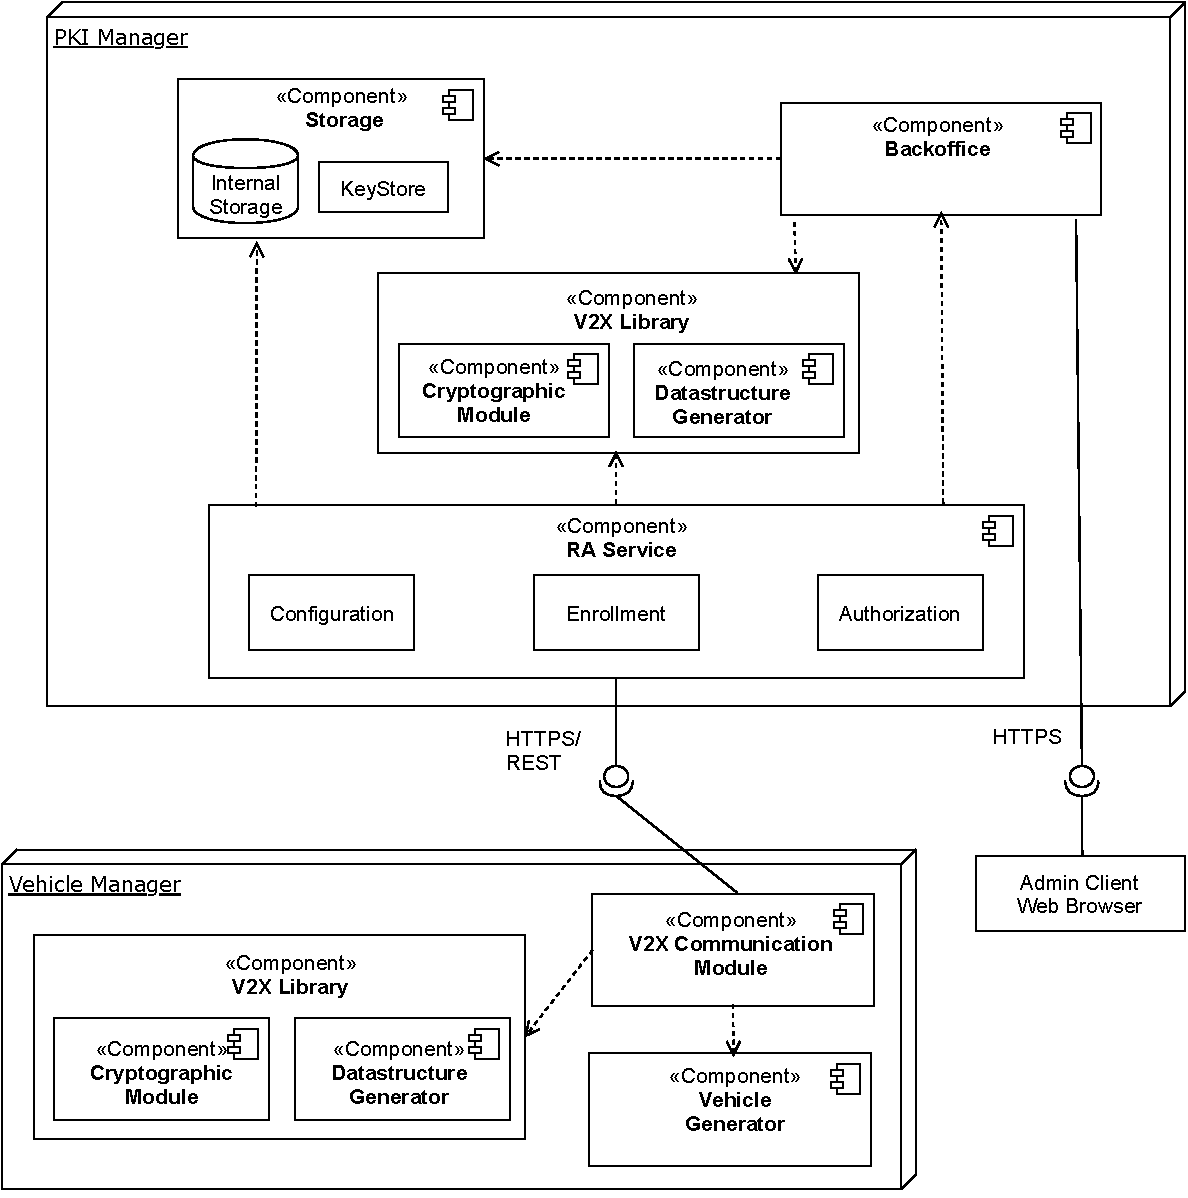
\includegraphics[width=0.8\textwidth]{Figures/architecture2}
	\caption{\label{fig:system_arch}Overall system architecture.}
\end{figure}

\subsection{System Components}

\paragraph{V2X Library}
\label{section:model}

The V2X Library is designed as a software library package. Its main goal is to create all the data structures specified in the latest version of the ETSI TS 103 097 standard. Such structures combine to form the certificates and messages that are used by the vehicles and PKI. In addition to this, the library also allows is users (PKI Manager and Vehicle Manager) to perform cryptographic operations related with the generation of certificates, signature of messages as well as their verification. The usage of this library allows the PKI Manager and Vehicle Manager to perform such operations in conformance with the approved standards and algorithms.

\paragraph{PKI Manager}
\label{section:model}

The PKI Manager is a web application that functions as a backoffice to the PKI. Such application aims to provide administrative services related to the creation and storage of the vehicular PKI. For example, it enables an admin user to log in and create new CAs, their cryptographic keys and certificates. The PKI Manager allows the creation and configuration of a new PKI or even change the structure of an already existent PKI. This application is connected to a database and keystore to provide persistence regarding the PKI information.


\paragraph{RA Service}
\label{section:model}

The RA Service is designed as an API (Application Programming Interface) of the PKI Manager, its main goal is to act as proxy between the vehicles of the Vehicle Manager and the CAs existing on the PKI Manager. The RA has two responsibilities: verifying the vehicle's identity and supporting their requests for enrollment certificates and authorization tickets. The former task requires the RA to perform an initial vehicle configuration, much like authentication, the goal is to “remember” and securely identify each connection to an already configured vehicle. The later task involves sending such requests to the correct CAs for certificate issuing and responding to the vehicles with the requested certificates. The RA Service uses encryption and digital signatures to ensure that the exchange of certificates is secure and the privacy of the end-entities is protected.

\paragraph{Vehicle Manager}
\label{section:model}
As the name suggests, the Vehicle Manager aims to manage the vehicles that will participate in V2X communication. This application runs on its own process and can be configured to create a given number of vehicles each as a client of the RA Service. Once created, the vehicles can contact the RA Service in order to request the end-entity certificates. Only with this initial configuration done, the vehicles are able to start communication with each other in respect to the Vehicle Manager configuration.

\subsection{Communication}
Now that we have seen components of the project and what they do individually, it is time we study how they interact with each other and how is the communication organized. 
As we can see from Figure \ref{fig:system_arch} we assume a client-server architecture, where the server is the PKI Manager and the Vehicle Manager acts as the client. On the server-side, the client requests will enter through the RA Service API, which then communicates with the back end and V2X Library to access the PKI services. As the RA Service is part of the PKI Manager project, the communication with the back end is achieved through simple service calls. Regarding the V2X Library, because this component exists on a different project we used it as a dependency of the server. The V2X Library is a Maven project, so it is possible to include it as one of the server's dependencies, which gives the server access to all the public classes and methods that the V2X Library has to offer. With this information is possible to create an interface on the server-side specifying the methods that will be used by the server as services of the Library. For example, generate a certificate or message, or verify them. Regarding the communication between the server and client, the HTTPS protocol is used to ensure protection of the sensible data that will be exchanged between them. Within the client, the same process is used for the usage of the V2X Library's services.



\subsection{Protocol} \label{protocol}
The interaction between the Vehicle Manager generated vehicles and the PKI is divided into several phases. For the definition of such phases, we assumed the vehicle's life cycle as defined in Section \ref{section:life-cycle}. Essentially, vehicles use the information installed at manufacture time to request the enrollment credential, later using this credential in order to request authorization tickets to start V2X communications. As seen in Figure \ref{fig:system_arch}, the only way that a vehicle can reach the CAs on the PKI Manager is through the RA Service. Specifically through the RA's services of \textbf{configuration}, \textbf{enrollment} or \textbf{authorization}, each of these services represents a phase in the vehicle to PKI interaction. The SSL protocol is used to secure the integrity, privacy and authenticity of the sensitive data that is transmitted during by the Vehicle Manager and RA Service communications.

\begin{figure}[t]
	\centering
	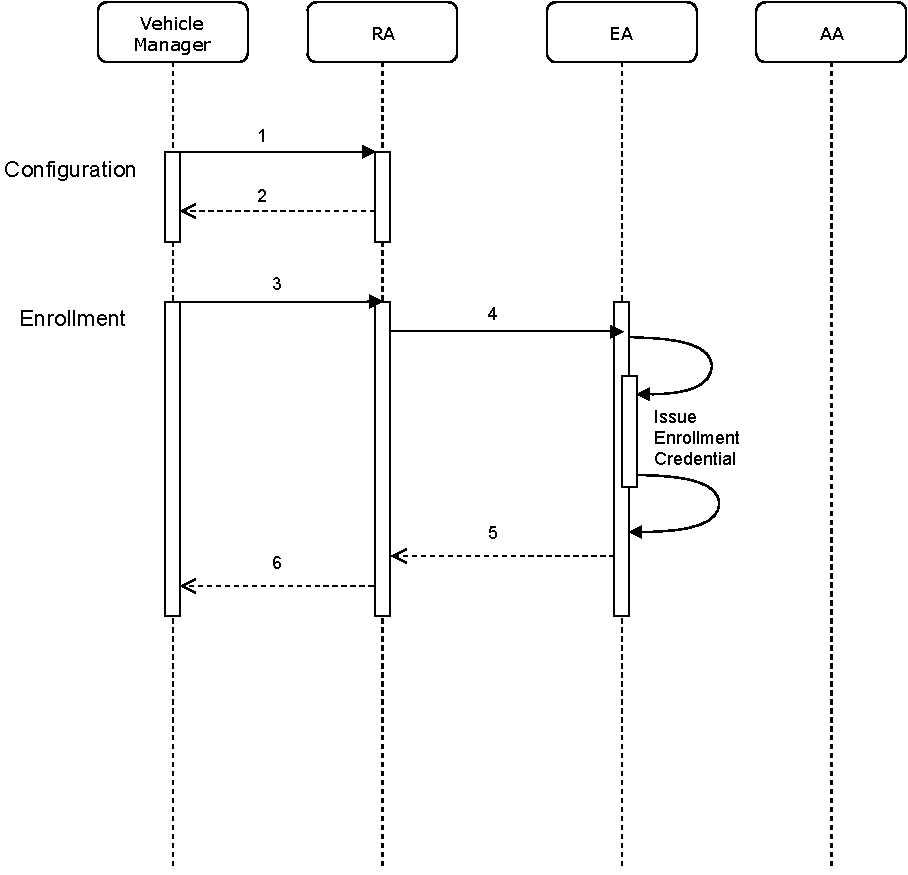
\includegraphics[width=0.8\textwidth]{Figures/protocolo_1}
	\caption{\label{fig:protocol_1}Vehicle configuration and enrollment process flow.}
\end{figure}

\subsubsection{Vehicle Configuration} \label{conf}
The first phase is the configuration. This phase aims to support the vehicle and RA configuration at vehicle manufacture time. Specifically, when the Vehicle Manager is generating new vehicles it uses this service in order to register them and to provide such vehicles with the information regarding the PKI. As we can see from message 1 to 2 represented on Figure \ref{fig:protocol_1}, first the Vehicle Manager starts this phase by sending message 1 containing the canonical public key and ITS identifier of a newly generated vehicle. The RA stores this information in its database and responds with the PKI information. The secure communication channel between the Vehicle Manager and RA Service allows the both RA to keep track of the trustworthy vehicles, and the vehicles to trust the PKI information which is responded by the RA. Such configuration will be the base of the trust that the RA has on the client vehicles for future interactions. 

\subsubsection{Vehicle Enrollment} \label{enroll}
The second phase is the enrollment. Vehicles which have completed the initial configuration can use this service to request the enrollment credential. To secure this type of communication we provide security at two levels: at the channel level through the SSL protocol and at the application level through the usage of digital certificates, signatures and encryption. Messages 3 to 6 represented on Figure \ref{fig:protocol_1} depict the communication steps of this service. The first step is made by the vehicle, in order to request the enrollment credential it first builds an enrollment request structure which is signed with the vehicle's private canonical key, and is encrypted for the attributed EA, see Section \ref{requests} for more information about the enrollment request structure. This request is the base of the application provided security. The second step involves the vehicle sending such request along with its secret identifier (ITS identifier) and the name of the attributed EA to the RA on message 3 through the SSL channel. Because the request itself is encrypted to the EA, the RA upon receiving it is not able to associate the vehicle's identifier with its future enrollment credential. Even so, the RA is able to perform the first vehicle identity verification. This is done by validating if the vehicle is already configured and is stored on its database. If this is the case, then the RA will send message 4 to the target EA. This message contains the encrypted request and the vehicle's public canonical key which will allow the EA to perform the second vehicle authentication verification. Unlike the first validation done by the RA which depends mostly on the security at the channel level, the second validation depends essentially on the security provided by the application. To do so, the EA first decrypts the request and validates the canonical signature made by the vehicle. Only if the signature is valid, it will issue the enrollment credential and include it in the response message 5. Such response is signed by the EA, encrypted to the vehicle and then sent to the RA which has the responsibility of returning it to the original vehicle using message 6.


\begin{figure}
	\centering
	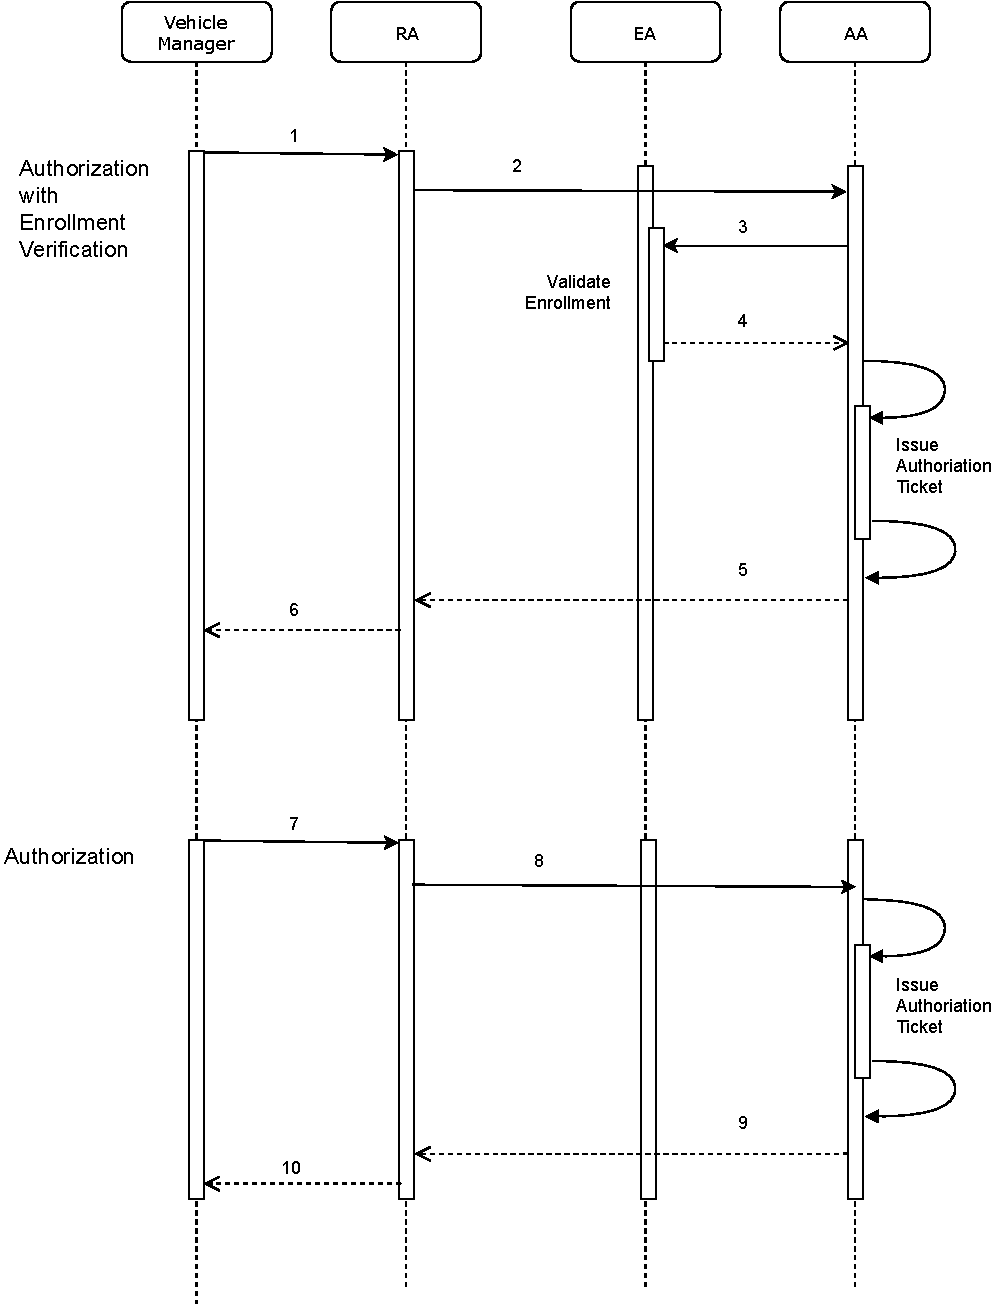
\includegraphics[width=0.8\textwidth]{Figures/protocolo_2}
	\caption{\label{fig:protocol_2}Vehicle authorization process flow.}
\end{figure} 

\subsubsection{Vehicle Authorization} \label{auth}
The last phase is the authorization which can be started by the enrolled vehicles. As the last phase, the security of this interaction is assured by the secure communication channel between the Vehicle Manager and PKI Manager, and by the application layer. Each time a vehicle requests one authorization ticket to an AA its enrollment must be verified. However, if such validation is performed by the AA the privacy of the vehicle would be compromised as the AA would have access to both the vehicle enrollment information (identity) and the pseudonym authorization ticket. To protect the vehicle's privacy, the enrollment validation is done by the EA which issued the vehicle's enrollment credential. Since a vehicle needs more than one authorization ticket, the consequence of this added privacy is the need to send more messages decreasing the performance of the vehicle authorization process as a whole. 

As we can see from Figure \ref{fig:protocol_2}, we have two flows from which a vehicle can request an authorization ticket. This enables us to leverage the RA in order to speed up the authorization process for each vehicle. The authorization process for a vehicle consists of multiple requests, if the vehicle is requesting the first authorization ticket the enrollment will be validated by the EA, otherwise the RA informs the AA that the vehicle's enrollment was previously validated. For the first authorization request, the vehicle starts by building the authorization request structure, such request contains all the information that the EA needs to validate the vehicle's enrollment status and that the AA needs in order to issue an authorization ticket. To ensure security and privacy in this type of communication, the vehicle's enrollment information such as its enrollment signature is encrypted to the EA and the authorization information encrypted to the AA. The vehicle sends message 1 containing the authorization request to the RA which knows how many requests the vehicle will perform during its authorization process. Message 2 shows the request being sent to the AA which decrypts it and sends the enrollment information to the EA in message 4. The EA decrypts its part of the request, validates the vehicle's enrollment signature, using the vehicle's enrollment credential (referenced by the request), and validates if such certificate is valid. If the verifications are in order, the EA sends message 4 which notifies the AA that the vehicle is authentic. The AA then issues the Authorization ticket, builds an authorization response structure which is signed, encrypted to the vehicle and sent to the RA within message 5 as a positive authorization.

At this point the RA knows that the vehicle is enrolled and that the authorization was successful, and is able to return the response to the vehicle in message 6. For the remaining requests the vehicle builds the authorization request and sends it to the RA as usual, as seen in message 7. The RA knows that the vehicle's enrollment has been validated for this authorization process and sends the request to the AA in message 8, the AA decrypts the requests, validates the authorization information, issues the authorization ticket, and returns the response to the RA in message 9. In the last step, message 10 shows the RA returning such request to the vehicle which stores the requested certificate. The same flow is repeated until the vehicle has all the authorization tickets for the time specified by the RA. 

\section{V2X Library}
As discussed before, one of the most basic concerns of this work is to implement a V2X ecosystem that is compatible with the most recent standardization efforts done by European organizations. In order to satisfy this requirement, the V2X library was implemented with ETSI’s standards in mind.
However, instead of blindly coding the information specified on the European standard we first searched for an already existing implementation. We found such a solution on the GitHub repository named C2C-Common \cite{c2c-common}, an open source Java package. However, upon closer inspection we noticed that C2C-common does not support the latest version of the European standard (1.3.1 at the time of this writing). In order to not reinvent the wheel, we decided to extend C2C-common by adding the necessary changes. In this section, we start by describing the detailed architecture of the library, then we take a look at the implementation of some of its most important data structures, and finalize by describing the services that our library provides. 

\subsection{Detailed Architecture}
The architecture of the V2X Library can be described as a layered structure, where at the highest level we can find the classes which allow the generation of the more specific data structures such as the EA, AA and Root CA certificates; vehicular authorization and enrollment certificates; and the V2X messages such as CAMs. As we go down a level the can find the more general substructures which the higher level structures depend. Finally, at the lower level we can find the classes which enable the transmission of such data structures in a cross-platform way.

As we can see from Figure \ref{fig:v2x_arch} the architecture of the V2X Library is divided in three layers. Starting at the layer 1 we have the super classes which are responsible to implement the Abstract Syntax Notation 1 (ASN.1) \textit{Canonical Octet Encoding Rules} (COER) as used by the ETSI standard. The ASN.1 is a standard description language for defining data structures that can be serialized and deserialized in a cross-platform way. ASN.1 is closely coupled with a set of encoding rues (e.g. COER) which specify how to represent a data structure (e.g. an integer) in a series of bytes (serialization) and vice-versa (deserialization). At this level, we can find the most basic of COEREncodable structures such as sequence, enumeration, choice, etc. as well as their implementation of the encoding/decoding methods. Such structures will be part of the V2X certificates and messages according to the specification of ETSI. Because the definition of these structures and the respective encoding/decoding implementations depend only on the version of ITU-T X.696 standard \cite{coer_standard}, change on the C2C-common library at such a low level was not needed. In addition to the implementation of the COER structures, it is at this layer that the V2X has performs the most basic cryptographic operations. Such operations include the digest, signature and encryption of data and will be used exclusively by the layer 2 in order to build the data structures which require them. For example, certificates and V2X messages are always signed, and certificate requests are both signed and encrypted. 

Going up a level we can find the sub-classes of the more general COER structures, for example, the certificate which is a child of COERsequence. This means that a certificate is just a sequence of fields (i.e. base data structures such as the host name, issuer identifier, duration validity, signature, etc) and should be encoded/decoded as such. Because the certificate and message structures depend on the version of the ETSI standard, it was at this level that we introduced more changes to this library. 

Besides updating C2C-common, our contribution also included the addition of a new set of standardized messages, the request for vehicle certificates. Such messages are encrypted and signed to assure confidentiality and authentication on the certificate request and deliver. In our case, they are used by the vehicle manager and RA. The specification of this data structures can be found in the ETSI's Trust and Privacy Management standard \cite{etsi_privacy} and follow the same COER encoding rules. 

At the layer 3 we can find the generator classes that the library user needs to instantiate in order to generate certificates, V2X messages and certificate requests. The generator classes are responsible to implement the certificate profiles for the different subjects and the different types of V2X messages for the vehicles. In addition to the generators, this layer also provides to the user the higher level cryptographic operations such as the validation of a V2X message, certificate, generation of a new keypair, etc. In our case, the generator classes and the user cryptographic module will be used by interfaces present on the Vehicle Manager and PKI Manager. 

To assure that every data structure is correctly implemented unit tests were performed to test the serialization and deserialization of the objects.

\begin{figure}
	\centering
	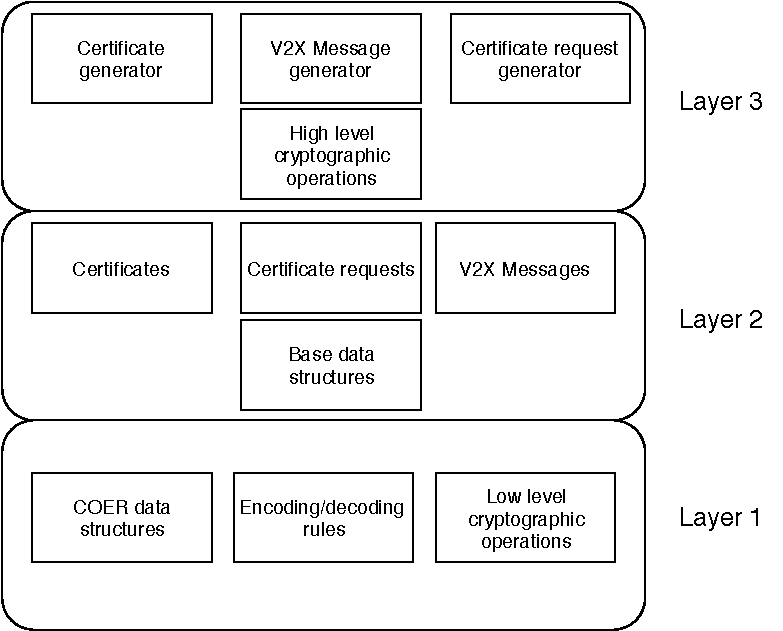
\includegraphics[width=0.8\textwidth]{Figures/v2xlib}
	\caption{\label{fig:v2x_arch} Layered structure of the V2X Library.}
\end{figure}

\subsection{The Data Structures}
We have seen how the library is organized, now we take a look at the implementation of the most important V2X structures. We start by describing the lower level COER structures, then we describe the higher level structures such as the certificate requests.

\subsubsection{COER Structures}
Before we can understand the higher level data structures, we have to understand the lower level COER structures which are part of them and therefore are the base of this library. All implemented data structures derive from the same type, the \textit{COEREncodable}, which allows us say that each can be encoded or decoded according to the \textit{COER} rules. In terms of implementation, this is enforced by the \textit{COEREncodable} interface which declares two methods, one for encoding and the other for decoding. This interface provides us with a solid base, as any class that implements it is able to provide its own implementation of the two methods. The classes which implement this interface are one level higher than the base type, they are the \textit{COER} structures. In this Section we describe the implementation of the most complex of such structures, the \textit{COERSEquence} and \textit{COERSChoice}. To understand the relation between the classes, Figure \ref{fig:coer_structures} provides a UML class diagram. 

\begin{figure}[t]
	\centering
	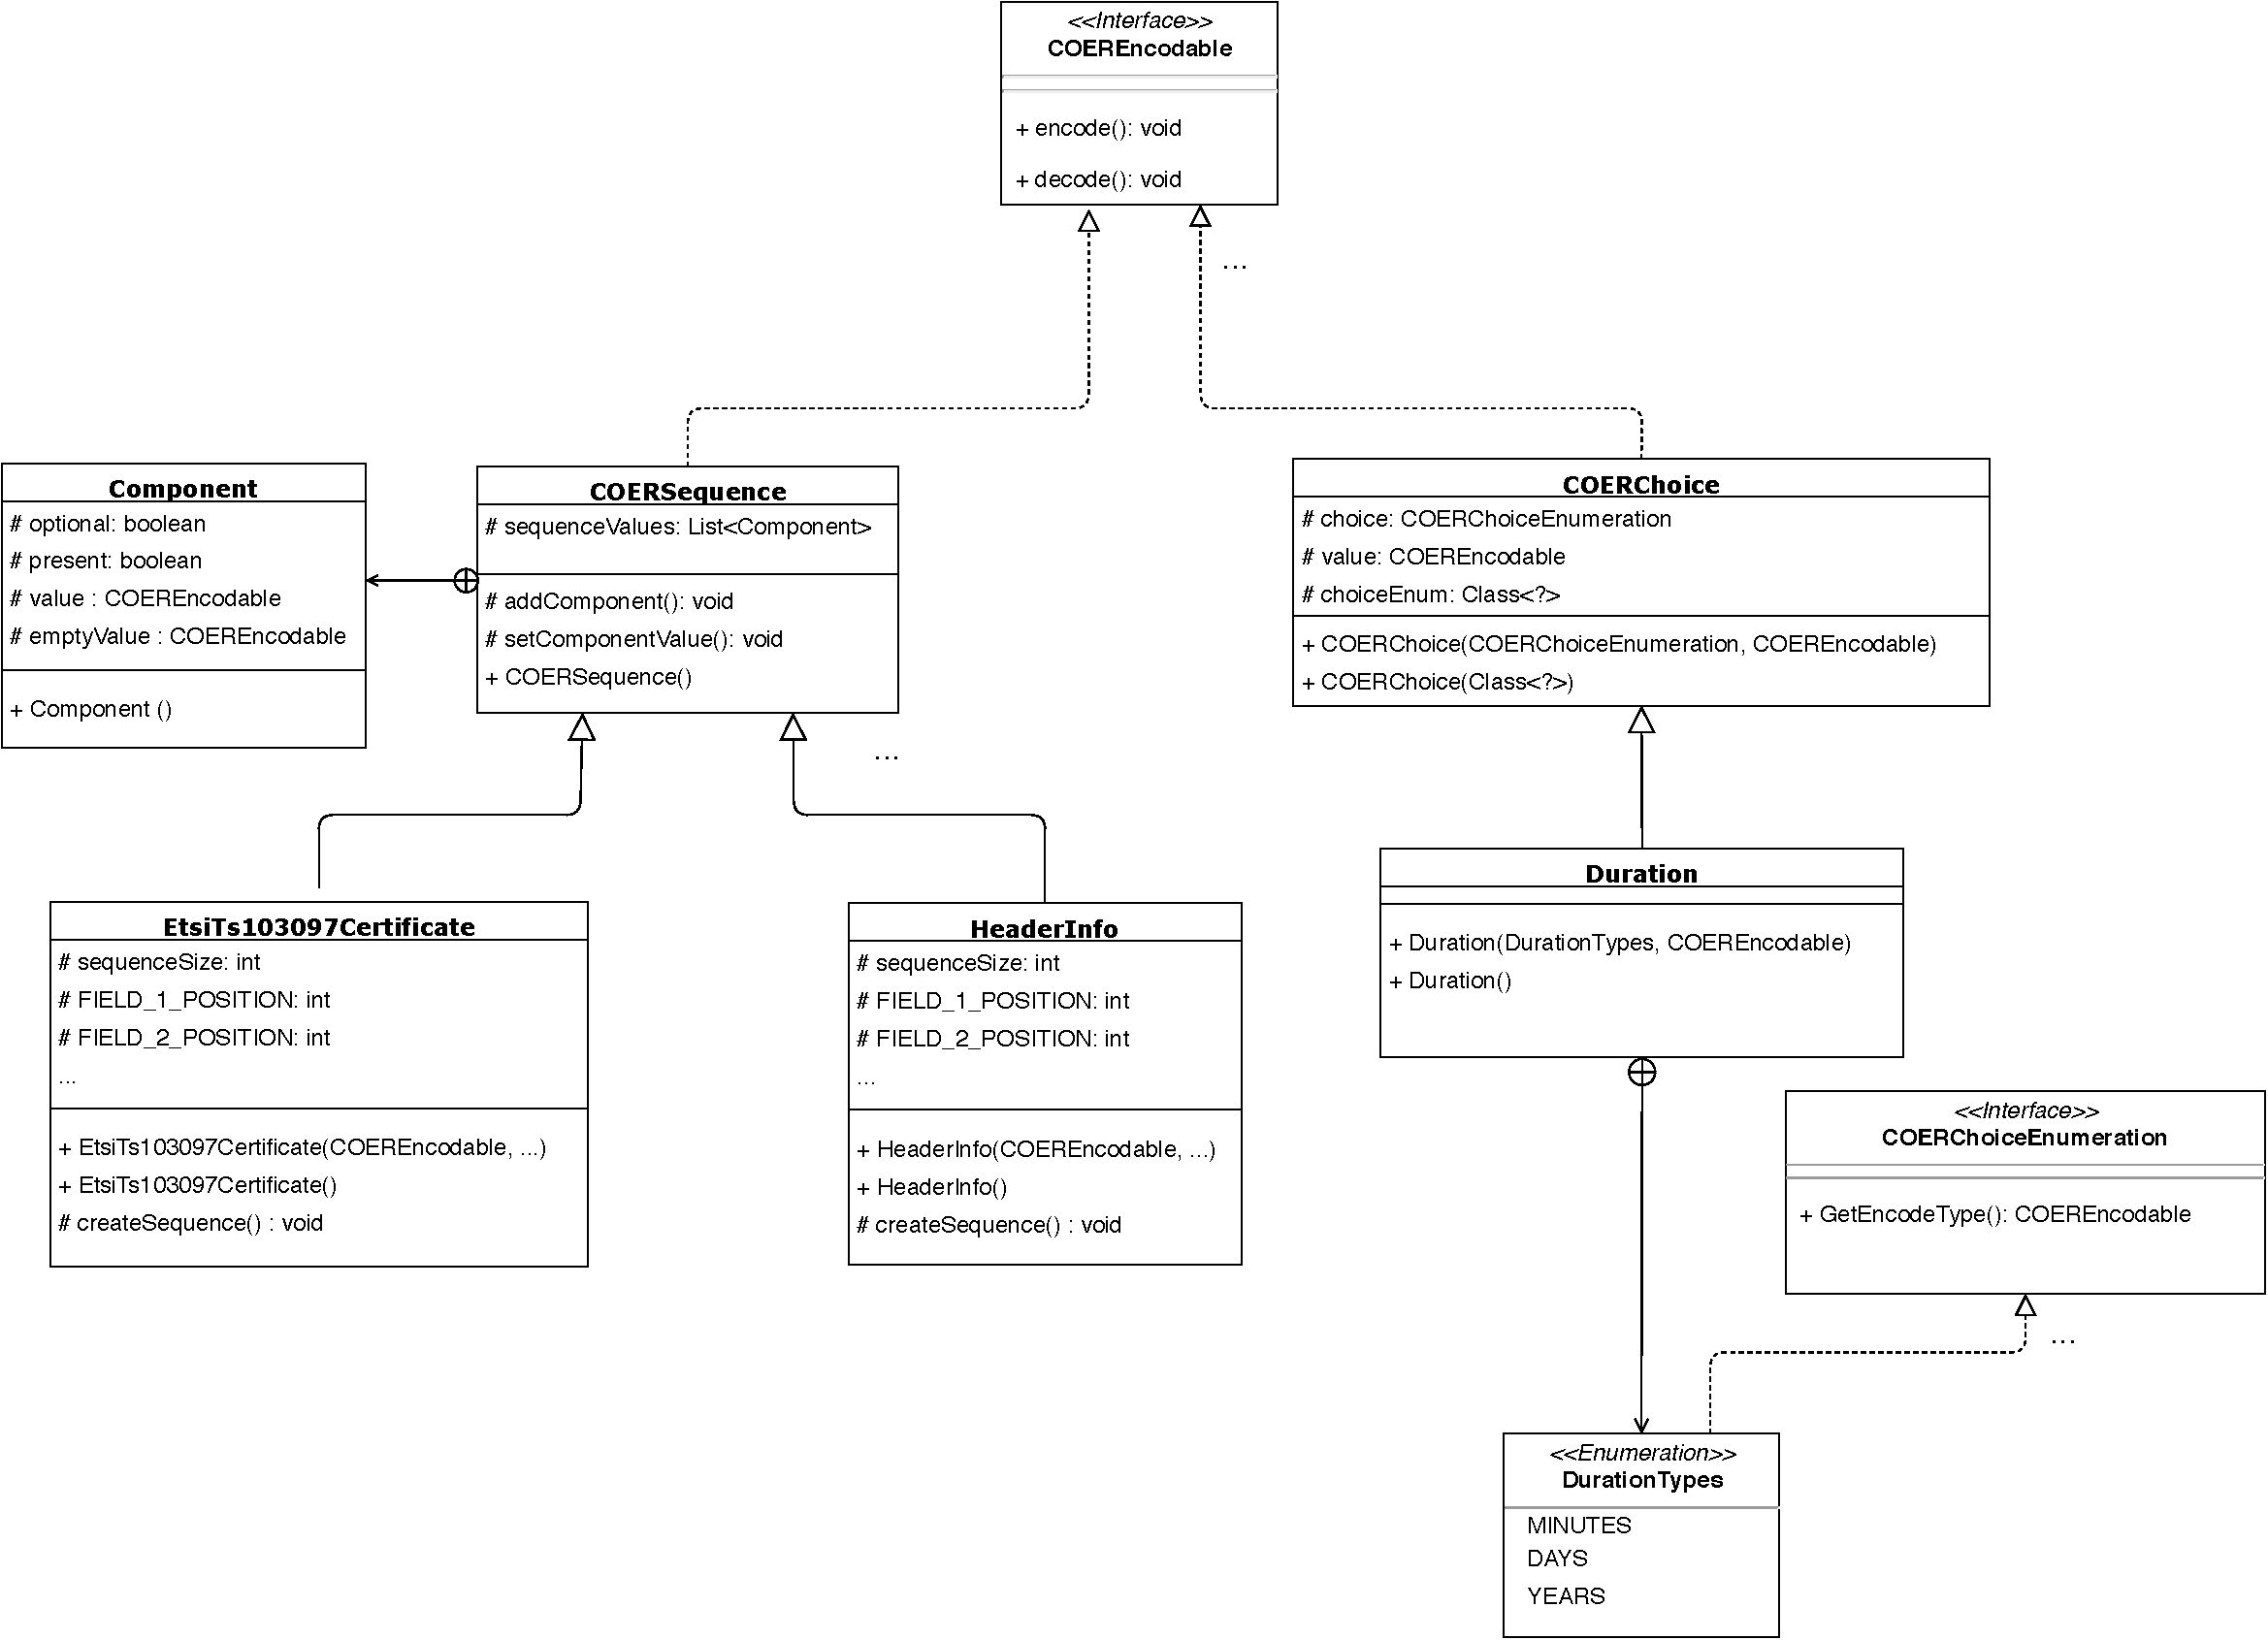
\includegraphics[width=1.1\textwidth]{Figures/coerstructures}
	\caption{\label{fig:coer_structures} Class diagram of the V2X {COER} structures.}
\end{figure}

\paragraph{COERSequence} The \textit{COERSequence} is a class which implements the encoding and decoding of a sequence of \textit{COEREncodable} elements. This class is very useful in the V2X Library as it allows us to combine a set of elements in a specific order to form a higher level data structure like a \textit{EtsiTs103097Certificate}. Generally speaking, the \textit{COERSequence} is a super class which provides the implementation of the \textit{encode} and \textit{decode} methods. Such class can be extended in child classes which can be seen as more specific types of \textit{COERSequence}, for example, the \textit{EtsiTs103097Certificate} which is an ordered sequence of certificate fields, and \textit{HeaderInfo} representing a specific sequence of header fields on a V2X message. Once an object of the sub class is instantiated it is possible to call the \textit{encode} or \textit{decode} methods to assure that the encoding rules are respected according to their definition on the super class. 

\begin{comment}
An object of a child class can be instantiated in two modes: for encoding or decoding a sequence. The general idea is that when an object of the subclass is created for encoding it initializes all attributes on the super class which are needed to encode it, making it possible to call the \textit{encode} method afterwards. When an object of the sub class is created for decoding it creates a placeholder object which then will be filled by the \textit{decode} method with a real values.
\end{comment}


In terms of implementation, the \textit{COERSequence} class represents an ordered sequence by having a list of \textit{Components} as a class attribute. A \textit{Component} is a helper class that represents a single component within the sequence. This class contains the to be encoded \textit{COEREncodable} value; a boolean variable representing if this value is optional; and an empty \textit{COEREncodable} object which indicates the type of the value in the decoding logic. This list of components represents the \textit{COERSequence} and is initialized by the class's constructor which receives the sequence's size in the parameters. The other classes that extend the \textit{COERSequence} are able to interact with such list during the process encoding or decoding an object. 

Before a sequence can be encoded it must be first populated, the \textit{COERSequence} class provides two methods for this effect: the \textit{addComponent} and \textit{setComponentValue}. The first method has the responsibility of creating the frame of the sequence, which is relevant to the decoding process to indicate the specific component type, position in the sequence, and whether the component is optional. The second method can be posteriorly called to add the sequence values to the frame, completing the creation of the sequence. It is possible to add a \textit{null} value in the sequence when the value is optional and not present. To minimize usage errors, \textit{setComponentValue} always checks if the mandatory components are present.



\paragraph{COERSequence Encoding}
The encode process starts when creating a sub class of \textit{COERSequence} (e.g \textit{EtsiTs103097Certificate}) using its dedicated encoding constructor with the sequence values as parameters. Each sub class maintains its own frame information such as the sequence size, component types, order and optionality. Because of this, when an object of the sub class is created for encoding the constructor is able to initialize the list of \textit{Components} within the super class. This process is achieved in three steps: first the super constructor is called with the sequence size, then the \textit{addComponent} and \textit{setComponentValue} methods are called for each sequence element with the respective frame information and value. Once the sub class object is created, it is possible to encoded it by calling the \textit{encode} method. This method receives a \textit{DataOutputStream} in which the encoded bytes will be written to. The encoding of a \textit{COERSequence} consists of a preamble followed by the encoding of each sequence element. The preamble is a stream of bits which allows specifying the presence of the optional elements in the sequence. Each present element (not null) is then encoded with respect to its type (e.g COERInteger, COERString, Signature, etc) in the order that they appear in the sequence. 

\paragraph{COERSequence Decoding}
The decoding process is similar to the encoding. Instead of calling the encoding constructor we call the decoding constructor to create the frame of the sequence within the super class \textit{COERSequence}. This is achieved by the decoding constructor in two steps: calling the super constructor with the sequence size, and the \textit{addComponent} method for each sequence element with its type, order and optionality. The result is the list of \textit{Components} on the super class containing the frame of the sequence but no values. We now have a \textit{COERSequence} sub class which is instantiated to be part of the decoding process. To do so, we just need to call the \textit{encode} method with the \textit{DataInputStream} in which the encoded values will be read from. The process of decoding starts by reading the preamble to identify which of the optional values are present. The next step is to decode each present sequence value into their original object. This is done by iterating through each member of the empty list of \textit{Components} and decoding it according to its type (represented by the empty \textit{COEREncodable} value). The final step is to set the \textit{Component} value to the obtained object. When the decode process finishes, the sub class will have access to the complete sequence in the \textit{COERSequence's} class list attribute.


\paragraph{COERChoice}
The \textit{COERChoice} is a class that implements the encoding and decoding of a choice of \textit{COEREncodable} elements. This class is very useful in the V2X Library as it allows us to specify the choice of one element from a set of known \textit{COEREncodable} values. Some applications include: the type of time duration on a certificate's validity (years, days etc.), the certificate's issuer identifier (self signed or digest of the issuer's certificate), and many others. 

Like the \textit{COERSequence} and all other COER classes, the \textit{COERChoice} is a super class which provides the implementation of the \textit{encode} and \textit{decode} methods. The process of encoding or decoding a choice starts when creating a child of the \textit{COERChoice} (e.g. \textit{Duration}) using the dedicated constructors. 


The objective of the encoding constructor is to initialize all the attributes on the super class (\textit{COERChoice}) needed for encoding. Such attributes include the choice and its value. To implement this, all sub classes contain a Java enumeration listing the possible choices for its type, for example \textit{Duration} contains an enumeration listing the possible types of time duration (microseconds, seconds, days and years). With this enumeration it is possible to instantiate a sub class object by calling the encoding constructor and passing an enum item which represents the choice and its corresponding \textit{COEREncodable} value. 

To uniformize the type of these enumerations through all the \textit{COERChoice's} sub classes, they implement the same \textit{COERChoiceEnumeration} interface. This enables the encoding constructor of the sub class to call the corresponding constructor on the \textit{COERChoice} passing the \textit{COERChoiceEnumeration} item and the value. An example of this interaction would be creating an object of \textit{Duration} with the \textit{COERChoiceEnumeration} item of \textit{YEARS} and the value of 4, representing a duration of four years. In this case the \textit{Duration} class encapsulates the value in to a \textit{Uint16} structure, an unsigned 16 bit \textit{COEREncodable} integer, and calls the \textit{COERChoice} encoding contrustor with the choice of duration (time unit) and the value. Thus, initializing the super class attributes for encoding and concluding the creation of the \textit{Duration} object. 


\paragraph{COERChoice Encoding}
To encode the created sub class object we simply need to call the \textit{encode} method, the implementation of this method exists in the super class because it is the same for all types which extend the base type of \textit{COERChoice}. In terms of implementation, the \textit{encode} method works with the attributes of the choice (\textit{COERChoiceEnumeration}) and value (\textit{COEREncodable}). The encoding consists in the creation of a \textit{COERTag} tag followed by the encoding of the \textit{COEREncodable} value. The tag allows the decoder to know the specific choice that the value belongs to, as it contains the position of the choice within its \textit{COERChoiceEnumeration}. This stream of bytes is enabled by the \textit{getOrdinal} method which is implemented within all \textit{COERChoiceEnumerations}, thus allowing the \textit{COERChoice} class to call it using its choice attribute. The \textit{encode} method then creates and encodes a \textit{COERTag} object with the ordinal value, encodes the \textit{COEREncodable} value (in the class value attribute), and finally appends it to the tag. The result is a stream of bytes representing the choice and the value.

\paragraph{COERChoice Decoding}
The process of decoding a sub class of \textit{COERChoice} is similar to the encoding, as it starts by creating an object of the sub class but calling its decoding constructor. Such method will initialize the choice attribute on the super class so that the value can be filled by the decoding process. This is achieved by calling the corresponding constructor on the \textit{COERChoice} class with the main type of the \textit{COERChoiceEnumeration}. For example, in the case of the \textit{Duration} class is the \textit{DurationTypes} enumeration which implements the \textit{COERChoiceEnumeration} interface. This will initialize the \textit{choiceEnum} attribute on the super class which is needed for the decoding process. Once the empty object is created (i.e. without the value), the \textit{decode} method can be called. Such method will first decode the \textit{COERTag} to get the specific choice from its \textit{choiceEnum} attribute. With the choice it is possible to get the \textit{COEREncodable} value associated to it, we just need to know its main type. This is achieved by the \textit{getEncodableType} method which is implemented within the \textit{COERChoiceEnumerations}, thus enabling the \textit{decode} method to use it on the recently discovered choice attribute. This method contains a switch that given the choice will return its intended main type. For example, in the \textit{DurationTypes} enumeration it will return an empty object of \textit{Uint16} since this is the type that represents the number of years, minutes, seconds, etc in a time duration. At this point the \textit{decode} method knows all the pieces to the puzzle and is able to decode the value by calling the \textit{decode} method for its main type. The application of this method will update the choice and value attributes of the \textit{COERChoice}, thus concluding the decoding. 


\subsubsection{Certificate Requests} \label{requests}
Besides updating the implementation of the certificates, V2X messages and all other data structures which they depend on, we had to implement the requests for vehicle certificates and their corresponding response. The specification for these data structures can be found on the ETSI's Trust and Privacy Management standard \cite{etsi_privacy} and they depend on the same \textit{COEREncodable} data structures as the V2X messages. 


\paragraph{Enrollment Request}
The first message that we implemented was the \textit{EnrollmentRequest} shown in Figure \ref{fig:enrollment_request}. This request contains two signatures and is encrypted to ensure the confidentiality, integrity and non-repudiation of the vehicle's important information such as the vehicle id, requested certificate attributes and the public verification which will be certified.

The request for an enrollment certificate is sent by the vehicles to an EA. In order to protect the privacy of the vehicles by hiding the vehicle's enrollment data such as ITS identifier this message will be encrypted with a symmetric key that is to be shared with the recipient EA. In terms of implementation, this message is an \textit{EncryptedData} structure which is a sequence that contains two elements: the recipient information and the ciphertext. The recipient information is the element that allows us to share the encryption symmetric key with the EA. This structure is implemented as a \textit{PKRecipientInfo} (Public key recipient information) containing the hash of the certificate that belongs to the recipient EA (\textit{recipientId}), and the 128 bit AES key encrypted with ECIES using the encryption public key of the recipient EA. The symmetric key is shared with the EA for of performance reasons, since encrypting large amounts of data with symmetric cryptography is faster than using asymmetric cryptography. For interoperability reasons, the encryption algorithms used are the ones approved by the standard. The ciphertext is the request's outer signature structure.

The outer signature exists to prove that the requesting vehicle has possession of the canonical keypair which was attributed to it when it was manufactured or the keypair of a current valid enrollment certificate. This allows the EA to trust that the origin of this request is an authentic vehicle, assuming that such key pair was securely stored by the vehicle's OBU. In terms of implementation, the signature is contained in a \textit{SignedData} structure which is sequence that also contains fields relevant to the signature's validation as well as the signed data. Specifically, this structure contains: the id of the hash algorithm used, signed data, signer information, and the signature itself. The signature over the to be signed can be calculated by two district ways depending on the vehicle's enrollment state: if this is the first enrollment request, the signature should be done with the vehicle's private canonical key; else it should be done with the private key of the currently valid enrollment certificate. To indicate the signature method, the field signer identifier is a \textit{COERChoice} which contains the hash of the enrollment credential in the case re-enrollment or empty otherwise. The data protected by the signature (signed data) is a sequence that contains a header and payload. The header is the data structure which contains information needed for the validation of the outer signature, it contains the \textit{Provider Service Identifier} PSID and the signature generation time. The PSID is a \textit{COERInteger} which identifies this message as a secured certificate request as assigned in the ETSI TS 102 965 standard \cite{etsi_PSID}. The payload of the outer signature contains the request's inner signature.

While the outer signature serves to prove the identity of the vehicle, the inner signature serves to prove that the requesting vehicles has position of the verification key pair which will be part of its enrollment certificate. In terms of implementation, the inner signature is very similar to the outer signature as it depends on the same sub structures. The only difference is that this signature is done using the vehicle's private verification key corresponding to the public key to be sent by this request. Therefore, the signer information field is always empty, indication that this is a self signed signature. The payload contains the data relevant to the emission of the enrollment certificate, this data is wrapped in a \textit{InnerECRequest} structure which is as a sequence containing: the vehicle's identifier, the version of the certificate standard, the public verification key, and the requested subject attributes. The requested attributes are the desired enrollment certificate attributes and contain data such as the enrollment validity period, region, desired application permissions, and the certificate subject name. 

\begin{figure}
	\centering
	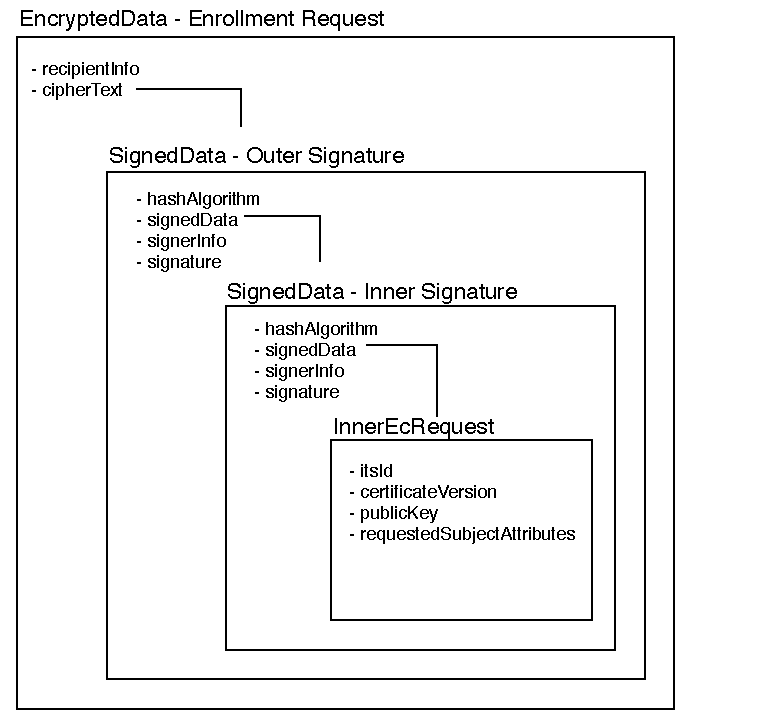
\includegraphics[width=0.8\textwidth]{Figures/enrollmentrequest}
	\caption{\label{fig:enrollment_request}Enrollment request message.}
\end{figure}

\paragraph{Enrollment Response}
The second request that we implemented was the \textit{EnrollmentResponse} shown in Figure \ref{fig:enrollment_response}. This message will be sent by the EA to the vehicle in response to its enrollment request. To protect the vehicle's privacy and securely deliver the enrollmnet certificate this request is signed and then encrypted. The request is encrypted using the symmetric key which was shared by the vehicle through the enrollment request. To indicate this, the recipient information is implemented as a \textit{PreSharedKeyRecipientInfo} structure which contains the hash of the AES key. The ciphertext of the encrypted data contains the enrollment response signature, which is done using the private key that is paired with the EA certificate's verification public key. This signature allows the vehicle to validate that the response originated from the correct EA. The signature protects the \textit{InnerECResponse} which contains the original request's hash value, a response code, and possibly the requested enrollment certificate. The hash value allows the vehicle to map this response to the original request by calculating and comparing its hash value. The response code indicates whether the request was successful or not. 

There are many possible ways which can cause the EA to decline the enrollment request, for example, if it can't parse the request, can't decrypt, the EA is not the recipient, invalid vehicle signatures, denied permissions, etc. To inform the vehicle of the problem, \textit{EnrollmentResonseCode} is a COEREnumeration which encodes the possible outcomes of the EA's enrollment validation. Only in the positive case the \textit{InnerECResponse} provides the enrollment certificate. 

\begin{figure}
	\centering
	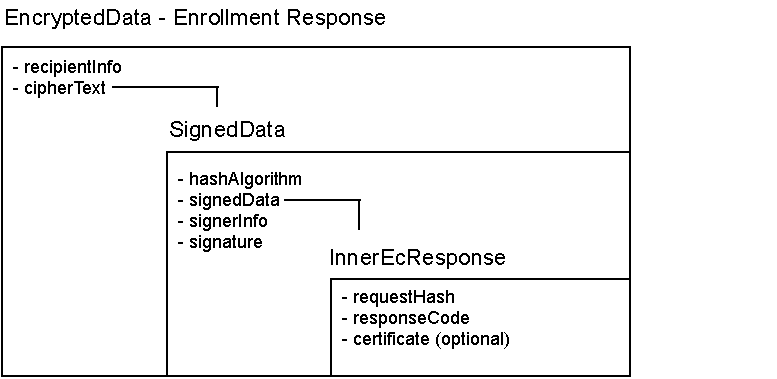
\includegraphics[width=0.8\textwidth]{Figures/enrollmentresponse}
	\caption{\label{fig:enrollment_response}Enrollment response message.}
\end{figure}

\paragraph{Authorization Request}
After we implemented the enrollment request and response we implemented the \textit{AuthorizationRequest} shown in Figure \ref{fig:authorization_request} since it depends on the vehicle's enrollment certificate. The authorization request is sent by enrolled vehicles to an AA which sends the enrollment certificate to the EA for vehicle enrollment validation. Since the authorization request includes the vehicle's enrollment certificate it introduces privacy concerns regarding the ability of the AA to link the enrollment certificate to the issued authorization tickets. To protect the vehicle's privacy the authorization request can be divided in two parts: the part which is encrypted to the AA and the part which is encrypted to the EA.

The process of encrypting the request for the AA is similar to the one used in the enrollment request since we are encrypting data to a certificate recipient. The authorization request is an \textit{EncryptedData} structure containing the recipient information and the ciphertext. While the recipient information contains the shared symmetric key which decrypts the request. The encrypted data is a \textit{SignedData} structure which ensures the AA that the vehicle is in possession of the verification key pair which will be certified by the authorization ticket. The signed data within this structure is the \textit{InnerATRequest} which contains the information that the AA needs to issue the authorization ticket and the information that the EA needs to validate the vehicle's enrollment. The \textit{InnerATRequest} is a sequence that contains: the verification public key, a \textit{ecSignature}, and \textit{sharedATRequest} structures. The \textit{sharedATRequest} is a structure which is to be shared between the AA and EA, it contains information that needs to be validated by both authorities in order to issue the authorizatio ticket. This structure contains the \textit{eaId}, allowing the AA to know which was the EA that enrolled the requesting vehicle; and the requested subject attributes which will be validated by the authorities. The \textit{ecSignature} contains the vehicle's enrollment credential signature, which is the part of the authorization request encrypted to the EA to ensure privacy in the enrollment validation. The ciphertext contains the signature computed with the private key corresponding to the enrollment credential of the vehicle. This mechanism allows the EA alone to decipher its part of the request and validate the vehicle's enrollment. To specify to the EA which enrollment credential was responsible for the signature, the field signder identifier contains the hashed vehicle's enrollment certificate. The signed data contains the hash of the previous \textit{sharedATRequest} since this structure is to be seen by both the EA and AA, therefore it can not be directly included in the encrypted \textit{ecSignature} structure. This external payload mechanism on \textit{ecSignature} allows it to ensure the integrity and non-repudiation of the \textit{sharedATRequest} while hiding vehicle's enrollment credential to the AA and still allowing it read the \textit{sharedATRequest}. 

\begin{figure}
	\centering
	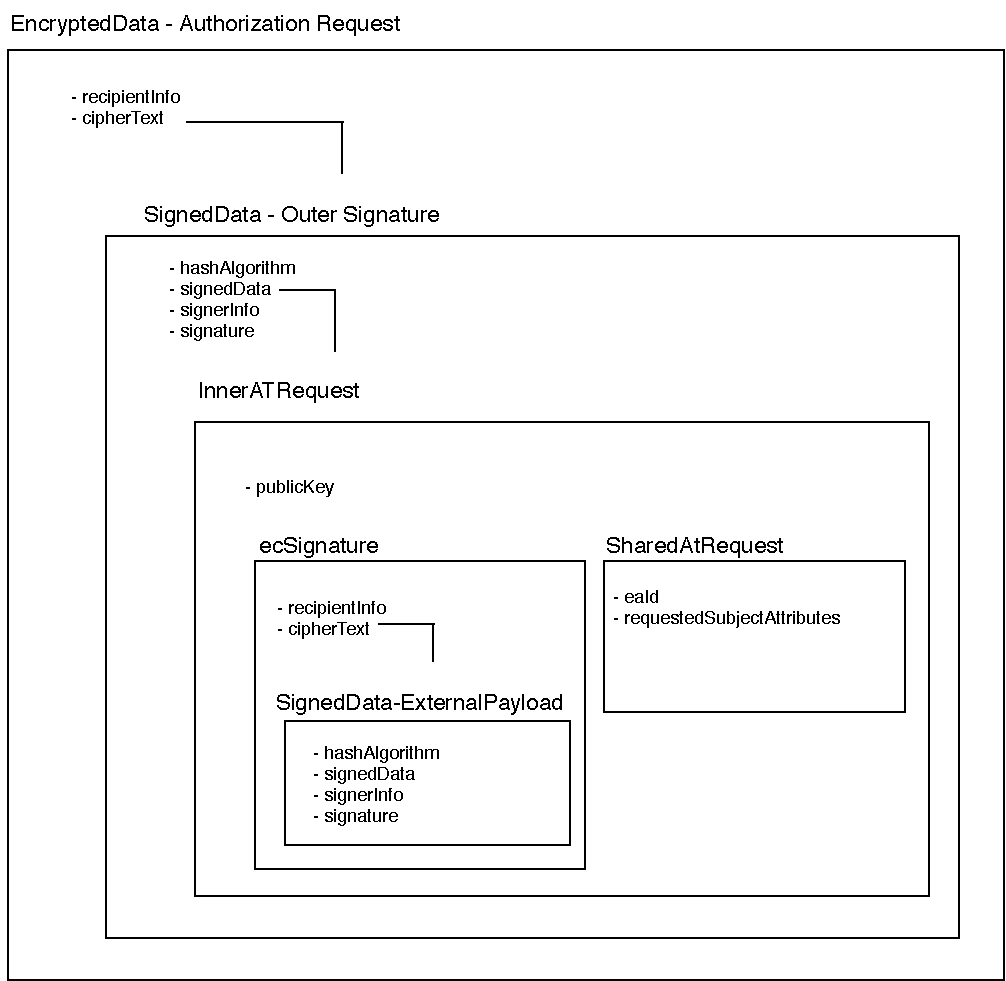
\includegraphics[width=0.9\textwidth]{Figures/authorizationrequest}
	\caption{\label{fig:authorization_request}Authorization request message.}
\end{figure}

\paragraph{Authorization Validation Request and Response}
These request/response messages are the intermediate step in the vehicle's request for an AT. To validate the vehicle's enrollment an \textit{AuthorizationValidationRequest} is constructed by the AA and sent to the EA. This structure contains elements from the Authorization request which was sent by the vehicle to the AA. Specifically, the \textit{ecSignature} and \textit{sharedATRequest}. The response is sent by the EA to the AA and contains the response code which will determine whether the AA is allowed to issue the AT or not. 

In terms of implementation the response is a \textit{AuthorizationValidationResponse} structure which is a sequence that contains the request hash, response code and the confirmed subject attributes. The request hash is SHA-256 digest of the \textit{AuthorizationValidationRequest} which will allow the AA to associate this response to its original validation request. The response code indicating the result of the EA's internal vehicle enrollment validation. In the positive case, the field confirmed subject attributes contains the subject attributes that the EA wishes to confirm; in the case that the EA denies the vehicle's enrollment the response code contains the reason, and the confirmed subject attributes is empty.

\paragraph{Authorization Response}
The \textit{AuthorizationResponse} shown in Figure \ref{fig:authorization_response} is the last message to be sent in the vehicle's authorization request. This message is sent by the AA to the vehicle and may contain the requested AT. To protect this response the message is signed by the AA and then encrypted such that only the original vehicle is able to decrypt. The encryption is similar to the method used in the enrollment response since a symmetric encryption key was previously shared by the vehicle with the AA in the Authorization request. The cipher text is a \textit{SignedData} structure which contains a signature done with the AA's private key that corresponds to its authority certificate. The signed data is the \textit{authorizationResponse} which contains: the request hash, allowing the vehicle to associate the AT request; the response code, which indicates the result of the authorization process; and the optional AT that is only present in the successful authorization case.
 
\begin{figure}
	\centering
	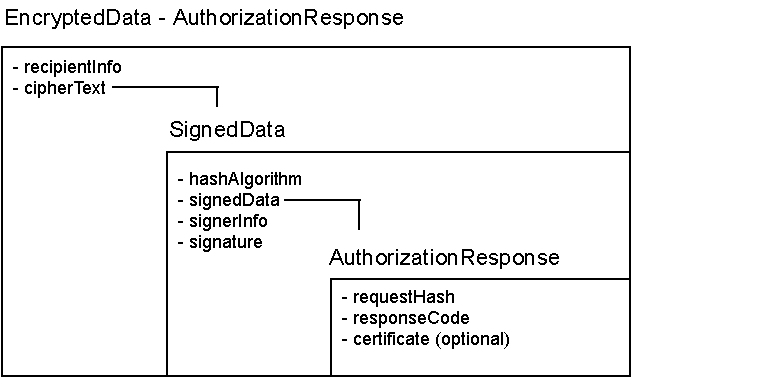
\includegraphics[width=0.8\textwidth]{Figures/authorizationresponse}
	\caption{\label{fig:authorization_response}Authorization response message.}
\end{figure}


\subsection{The Cryptographic Tools}
When privacy and security are requirements of a system, the use of cryptographic tools is essential. Such tools allow us to keep the information confidential thorough communication, to verify its integrity, freshness and authenticity.

The process of providing the secured data structures to the other system components implies that it is this library’s responsibility to perform the needed cryptographic operations in order to generate them. To facilitate interoperability between other potential systems, it is essential that such operations are performed according to the algorithms described in the latest version of the IEEE 1609.2 standard, which are also used by ETSI 103 097.

At a low level, the V2X Library uses Bouncy Castle as a security provider for all of its cryptogtaphic operations. Such API pvoides us with the implementation of the cryptogaphic algorithms allwoing us to abstact from their complex implementation details when performing cryptographic operations.
The V2X library contains within its functionalities the following cryptographic operations: 

\begin{itemize}
	\item The generation of symmetric and asymmetric keys. This operation must be called providing one of the supported key generation algorithms.
	\item The signing of data. This operation must be called providing a supported elliptic curve signing algorithm, the data to be signed, the signing certificate, and the signing private key. The result is a \textit{Signature} structure as defined in the European standard. 
	
	\item Verification of a digital signature. This operation must be called providing the data to be verified, the \textit{Signature} data structure, and the signing certificate with the correspondent certification chain. This function returns a Boolean value corresponding to the validation result. 
	
	\item Asymmetric encryption of symmetric key. Encrypting large amounts of data with asymmetric keys is inefficient, this should be done using symmetric keys. However, in order to decrypt a symmetric encrypted message, its recipient must have access to the same secret key (i.e. symmetric key) which encrypted the message. This operation exists to assure confidentiality in the process of sharing a secret key with a specific recipient. It should be called providing the secret key that will be encrypted, a supported elliptic curve encryption algorithm, and the public key of the recipient. 
	
	\item Asymmetric decryption of symmetric key. This operation must be called providing the encrypted symmetric key, the recipients private key and the elliptic curve decryption algorithm.
	
	\item Symmetric Encryption of data. This operation should be used to encrypt data with the \textit{AES CCM mode} algorithm, to call it we need to specify the data to be encrypted, the secret key and a nonce. The last parameter is to be used as input to the initialization vector for the encryption algorithm.
	 
	\item Symmetric Decryption of data. This operation must be called providing the encrypted data, and the decryption key and nonce which was originally used to encrypt the data. 

	
\end{itemize}

All of these operations are available at the Crypto Manager which was implemented as the default cryptographic module of V2X Library. It is also possible to extend the Crypto Manager in the future by adding new operations or support for new algorithms.


\section{PKI Manager}
Certificate issuing is an essential part of this work, however due to time constraints we were not able to extend mPKI. Our solution to this problem was to create the PKI Manager, a web application that functions as a demo PKI. 

The PKI Manager contains a backoffice which was implemented with the sole purpose of demonstrating the creation of vehicular certificates. However, it is much more limited comparing to mPKI. In the PKI Manager all the cryptographic operations related to the generation of keys, certificates and messages are done using software (V2X Library). 

Such operations share the processing resources with the machine which the PKI Manager is deployed, which can cause the entire machine to slow down and decrease the performance of the PKI Manager. In terms of security, these operations are only secure as the rest of the machine. A single security flaw in the operating system can compromise the security provided by the software encryption. In addition to the constraints in performance and security, the PKI Manager is also limited in terms of functionality. Although it provides the most basic vehicular PKI operations such as the enrollment, re-enrollment and authorization of vehicles it does not support the revocation of the certificates which belong to the end entities and CAs though a CRL mechanism. In this section, we describe the application, the technologies adopted, the features that it provides, and our implementation decisions.

\subsection{The Technology}
The PKI Manager is a web application implemented using the Spring Boot framework. This framework produces a stand-alone application and aims to reduce the time spent configuring it. This is achieved automatically by Spring based on the dependencies added to the project. For example, if we add a dependency that relates to a database, Spring will attempt to auto configure the application for database access.

These applications run on an embedded container, which simplifies the deployment process of the web application. We simply need to press the “start button” and access the application at the address indicated by \textit{http://localhost:8081/}. This is done by Spring, because we added the spring-boot-starter-web dependency it pulls the spring-boot-starter-tomcat automatically which in turn starts Apache’s Tomcat Web Server when we run the main method.

Our web application is organized as a Spring Web MVC application, this framework is a module of Spring that specializes in aiding the development of web applications. It provides all the functionalities needed to receive HTTP requests, delegate their processing to other components, and finally, build a response. MVC is an acronym for model, view and controller each name represents a fundamental part of a Spring Web MVC application. In order to understand each part, I will describe the basic flow of an HTTP request from the point of view of the Spring MVC.

When we access a URL in the browser that sends an HTTP request to our server, for example our \textit{http://localhost:8081/}, the framework will try to find a class that is responsible to deal with such request, delivering to it the data that originated from the bowser. This class is an application controller. The controller then passes the data to a model, which executes the necessary business logic such as validation, calculations or database access. The result of the operations is returned to the controller, which in turn returns the name of the view along with the data needed to render the web page. Finally, the framework tries to find the specific view that is responsible to process such data into an HTML page and returns it to the browser. 

In regard to our application's identity management and user authentication we decided to use Spring Security since it is also a module of Spring. By using a configuration file, we can limit the web pages which the users and administrators can access while authenticated. This feature allows us to protect services and information from unauthenticated parties. The PKI Manager authentication is done using the usual username and password method. In this approach, the server stores the username and the hashed value of the password in its database. In addition to storing user credentials, the database also stores the role of each user allowing us to differentiate the privileges for the different types of users (regular user or admin). 

\subsection{The Database}
One of the concerns that we had when creating the PKI Manager was the persistence of the PKI information. We decided that even though this PKI exists for demonstration purposes, it would be important to store it in a non-volatile way. This decision allows us to keep consistency of the PKI even if the server crashes/restarts. In this section we describe the data access layer of the PKI manager, we start by introducing the technologies adopted, then we take a look at the design of the database. 

\paragraph{The database technology}
The database service is provided by PostgreSQL, a relational database management system. A database server runs locally, to which our application connects at the start of its execution.

The database access is provided by another of Spring's modules, the Spring Data JPA. This framework aims to simplify the data access layer of the applications by reducing the code needed for its implementation. To do so it relies on the entities and repositories. The entities are classes which correspond to tables in a database and are created with the help of the Spring annotations. It is through these annotations that we can specify the name of the table, its columns, primary keys, the relations between tables, etc. While the JPA entities allow us to shape the diagram of the database, the repositories provide us with a way to interact with it using queries. To be precise, these repositories are divided in two parts, the Repository and the Repository interface. The Repository is a class implemented by Spring, it has direct access to the database and queries it. The Repository interface is an abstraction of the Repository in which the developer can add methods in order to specify the supported queries. This can be done in different ways, for example, it is possible to create a query from the method's name or using Spring annotation. In our case, we used the first method for the more simple queries, and provided Spring annotation containing a native SQL query to support the most complex of the database queries. 

\paragraph{The database design}
To provide persistence with regard to the PKI Manager, we designed a database which keeps the information about the PKI entities and the operations of the PKI Manager. To minimize redundant data and facilitate finding information, we introduced relations between these PKI entities naturally. Figure \ref{fig:database_diagram} shows the entities that we took into account, their characteristics and relations.


\begin{figure}
	\centering
	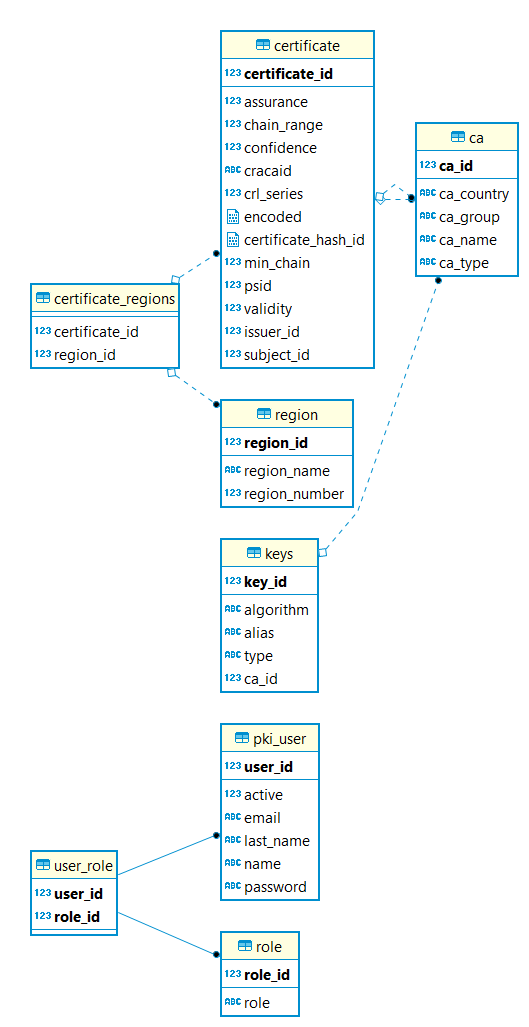
\includegraphics[width=0.8\textwidth]{Figures/db_diagram}
	\caption{\label{fig:database_diagram}Database entity relation diagram.}
\end{figure}

As we can see from the Figure, the database stores in its tables information to support the user authentication and management of the vehicular PKI. Regarding the PKI information, it has a table for the CAs, keys, certificates and regions. 

The \textit{ca} table contains generic CA information such the CA type (Root, AA, EA), group (Root CA or Sub CA), name, and country. It is possible for a CA to have one or more keys associated, this is expressed by the one-to-many relation between the \textit{ca} and \text{keys} tables. Regarding the relations between CAs and certificates, we assumed two occurrences: A CA can be subject of a single certificate and the issuer of one or more certificates. These relations are expressed by the one-to-one and one-to-many relation between the \textit{ca} and \text{certificate} tables.

The \textit{keys} table contains generic Key information but not the key itself, this is because the key is stored in a keystore. We only use this table to store information needed to locate the key in the keystore and view its characteristic, such as the alias, type of the key (encryption or signature), the algorithm. The foreign key \textit{ca\_id}, allows us to know which CA a specific key belongs to. 

Because currently there is not a keystore that supports the storage of this type of CA certificates, we decided to store them in the database. The \textit{certificates} table stores all the information that we need to pass to the V2X library in order to generate CA certificates. The foreign keys \text{subject\_id} and \textit{issuer\_id} allow us to know which CA is the subject and issuer of a specific certificate. 


\subsection{The Backoffice}
The PKI Manager is accessible through the browser only by system administrators. This backoffice application uses the V2X Library and through its services provides a GUI where administrators can visually create and configure a demo vehicular PKI. In this section we describe the functionalities and implementation details of the PKI Manager.

Upon logging in, the administrator will have the option of managing the CAs, keys, certificates, or viewing the PKI dashboard. These operations can be chosen from the index page, each having a dedicated web page. Performing a PKI operation updates the application dashboard, shown in Figure \ref{fig:manager10}, allowing the user to understand the state of the PKI. Specifically, whether the PKI has the necessary CAs and if each is ready to issue certificates. On the ramining of this section we take a look at the steps which an admin user has to take in order to create a PKI using our backoffice application.

\begin{figure}
	\centering
	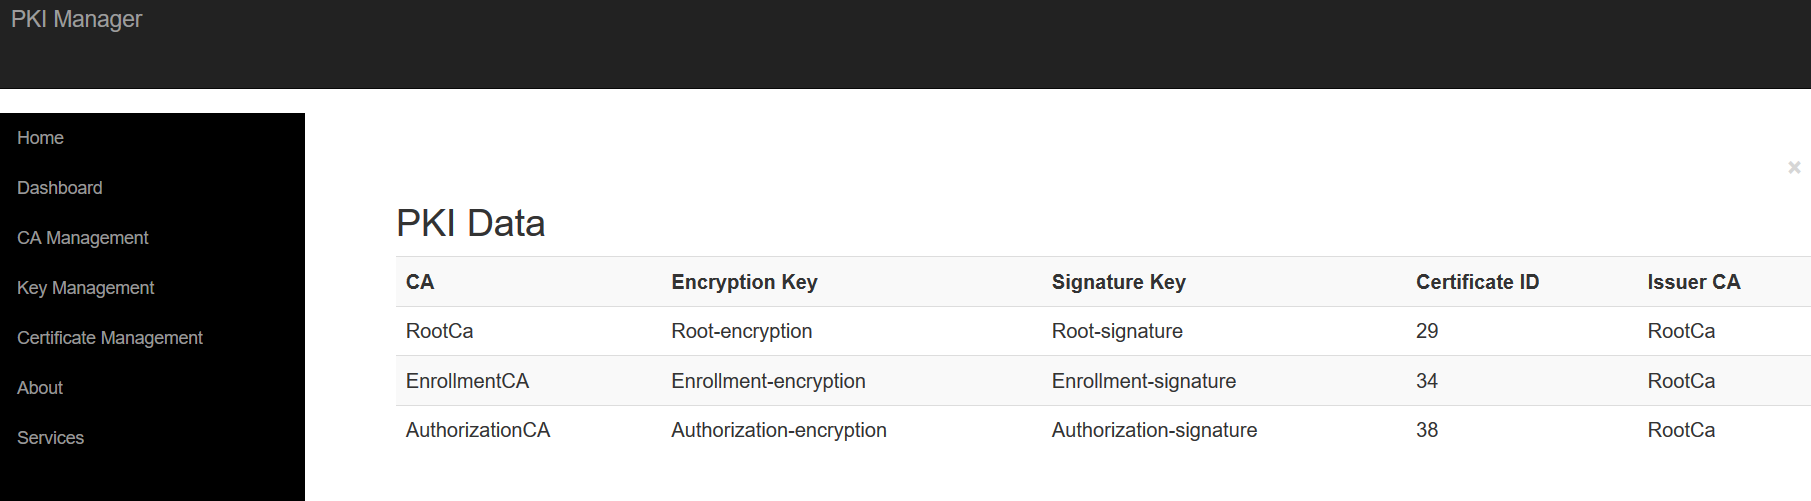
\includegraphics[width=0.8\textwidth]{Figures/manager10}
	\caption{\label{fig:manager10} Data of the created PKI}
\end{figure}

\paragraph{CA Management}
The first operation that should be done to have a functional PKI is the management of the PKI CAs. In this page, the user has the option of creating a CA by clicking a button. Performing this action displays the submit form shown in Figure \ref{fig:manager1}. In this form the user can specify the name, country and type of CA. The last is a drop down menu which shows the already defined CA types of Root, Enrollment and Authorization. When this form is submitted, this page's Spring MVC controller at the server-side will handle the POST request by storing the CA information on the database. To be precise, our controller calls the \textit{caManagementService} which performs the bussiness logic such as validation of the inputed information, then the service calls the \text{caRepository} that stores the information. When this logic is completed, the controller will redirect the browser to same CA management page, which makes it perform a GET request. The GET controller for this page will then handle such HTTP request by getting all the existing CAs from the database, returning them along with the requested web page to the browser. With this information it is possible to display the existing CAs as we can see from Figure \ref{fig:manager1}, updating the table each time we get the CA management page. 

\begin{figure}
	\centering
	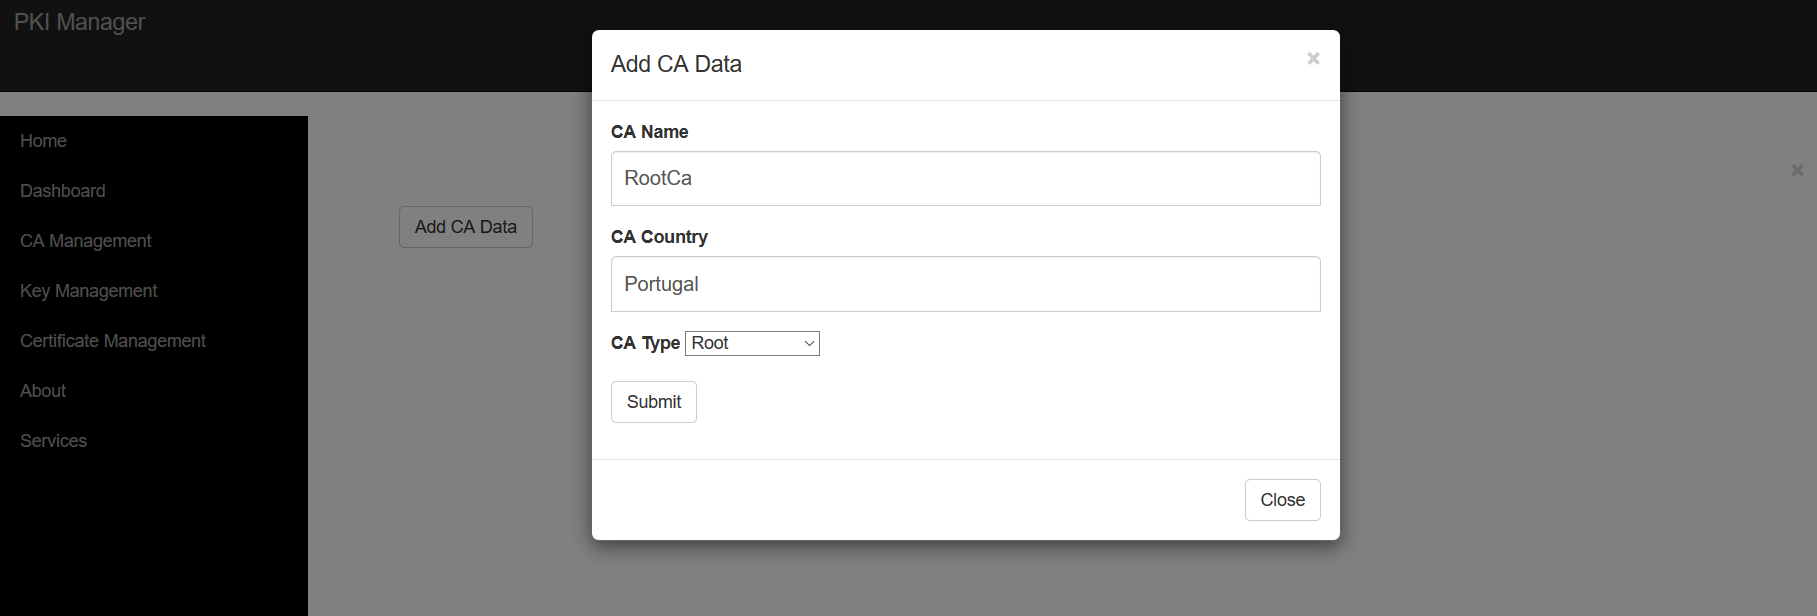
\includegraphics[width=0.8\textwidth]{Figures/manager1}
	\caption{\label{fig:manager1}From to add a new CA.}
\end{figure}

\begin{figure}
	\centering
	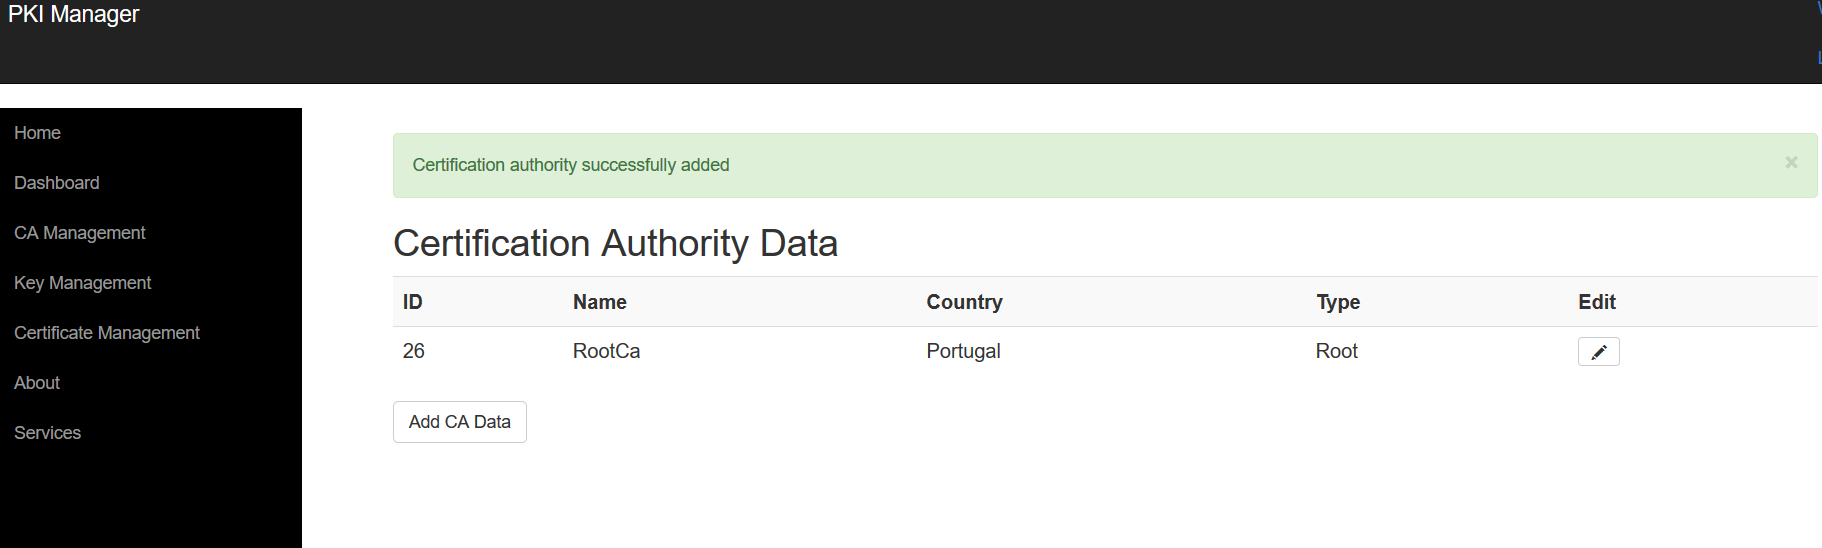
\includegraphics[width=0.8\textwidth]{Figures/manager2}
	\caption{\label{fig:manager2}Certification authority table.}
\end{figure}


The same logic is done for all the other operations, for each operation we have a spring controller which implements end-points that will handle HTTP GET and POST requests. The GET end-point has the responsibility of returning to the browser the web page with all the information needed to perform the operation. The POST end-point has the responsibility of generating resources (web pages, database information, services, etc.) on the server-side in respect to the information sent by the browser.

\paragraph{Key Management}
After creating a CA, the next step is to generate its signing and encryption keypairs. Once on the Key Management page, the user is able to do so by clicking a button. This button opens a form where the key alias, algorithm and owener CA can be chosen, as we can see in Figure \ref{fig:manager3} . In terms of constraints for these inputs, the alias must be unique, the user must select one of the provided encryption or signing algorithms, and one of the created CAs as the owner of the keypair. Being that these selectable values are loaded by the server in the browser when it requests this page. Submitting the form will send a POST request to our server, which will generate the key given the algorithm and store it with respect to the owner CA. The generation of the keypair is done using V2X Library interface which allows the PKI Manager to access the services of this library. The storage of the keypair is done regarding two aspects, the generated keypair and its information. The keypair itself is stored on a keystore file which is loaded into our server when its execution starts. The keystore data which is inputted by the user at the client-side is stored on the database. With this method it is possible to quickly search for a key in our database using its information and then find its value on the keystore providing the alias. Upon finishing these operations, the server will refresh the Key Management page, updating the existing keys table with the new entry.

\begin{figure}
	\centering
	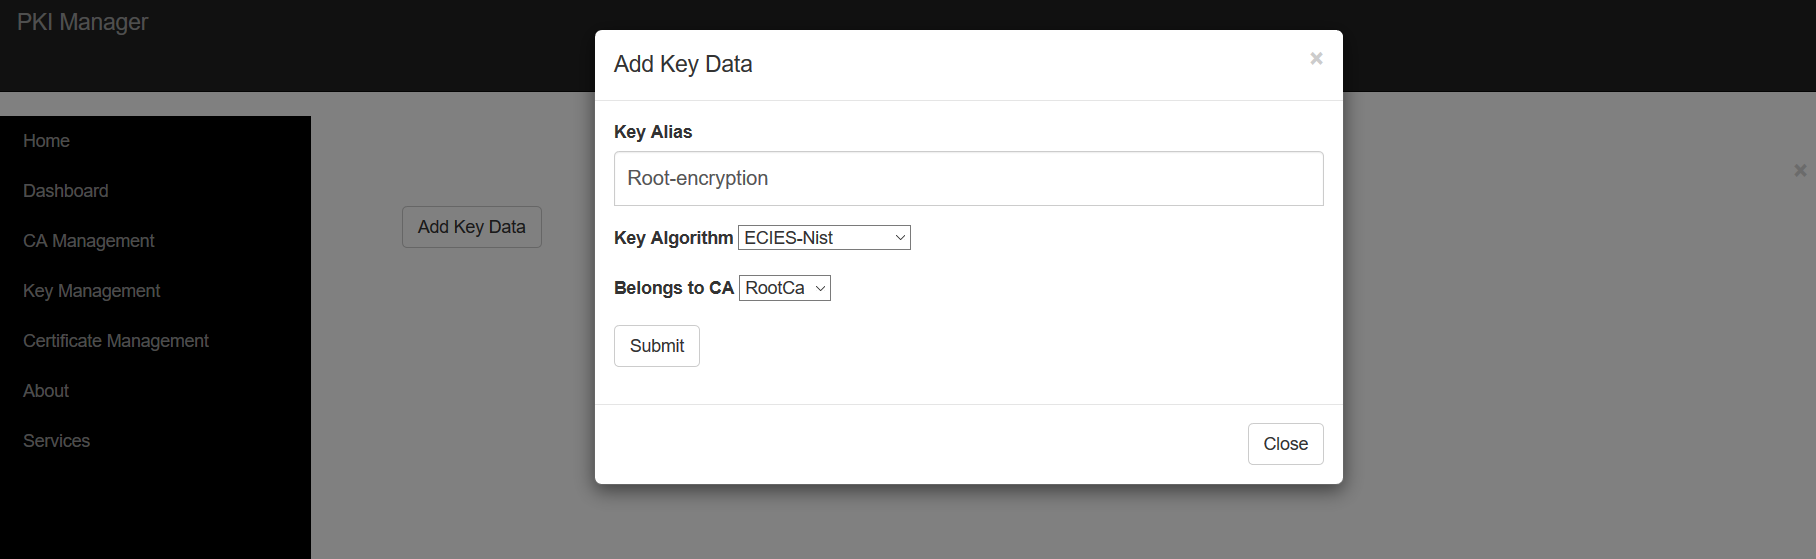
\includegraphics[width=0.8\textwidth]{Figures/manager3}
	\caption{\label{fig:manager3}Form to add a new keypair to an existing CA}
\end{figure}

\paragraph{Certificate Management}
The last step to have a functional CA is to generate its certificate. The Certificate Management page can be navigated to for this purpose. Once there, the user can generate a Root CA certificate or a Sub CA certificate by clicking the respective buttons. Generating a Root CA certificate involves filling the form shown in Figure \ref{fig:manager7} with the following information relative to the root certificate: time validity, country, and the Root CA which is the subject of the certificate. For the subject input the user is able to choose a CA from a list containing all the existing Root CAs which already have associated a signing keypair but no certificate. The list is provided by the server when the page is loaded and negates the user error of creating a certificate for a Root CA which is not ready to self-sign its certificate. Creating a Sub CA certificate is a very similar process with the difference that the user must fill the form displayed in Figure \ref{fig:manager8}. In this form the user must not only specify the subject of the certificate but also issuer CA. For the certificate's subject, a Sub CA with signature keys and no certificate must be selected. The issuer must be a Root CA which is ready to issue the certificate, i.e. a Root CA which has already has a signature keypair and a certificate associated. The mapping between a certificate and its issuer will allow the PKI Manager to build certification chains in the future. When the form is submitted, our server will compile the information inputted by the user, calling the V2X Library to issue the certificate and storing it on the database. Once these operations are finished, the server will refresh the Certificate Management page, updating the existing certificates table with the new entry. 

\begin{figure}
	\centering
	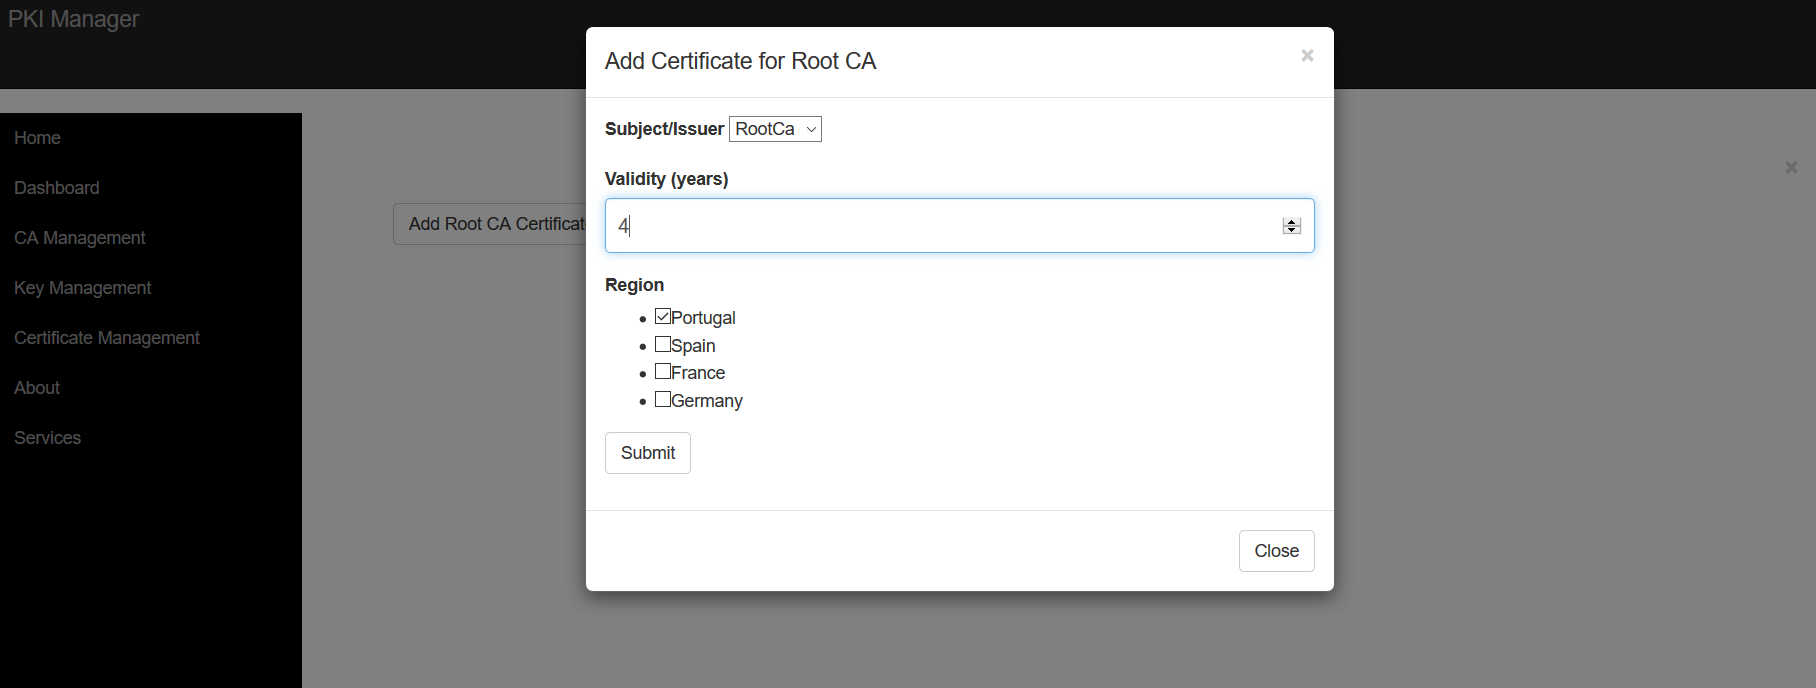
\includegraphics[width=0.8\textwidth]{Figures/manager7}
	\caption{\label{fig:manager7}Form to add a certificate to an existing Root CA}
\end{figure}

\begin{figure}
	\centering
	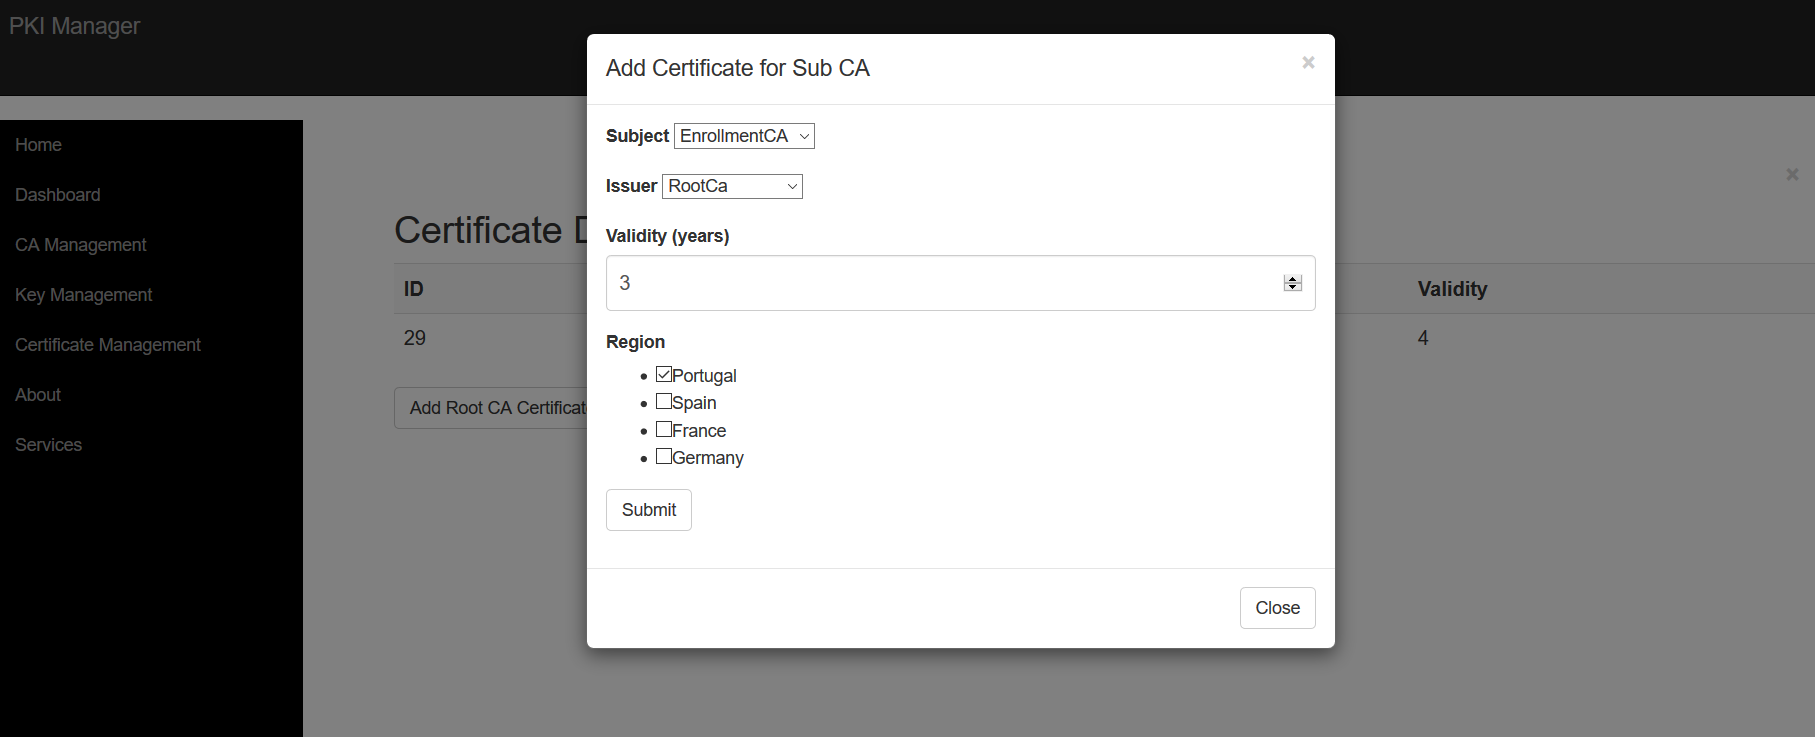
\includegraphics[width=0.8\textwidth]{Figures/manager8}
	\caption{\label{fig:manager8}Form to add a certificate to an existing Sub CA}
\end{figure}

\section{RA Service}
The RA Service can be seen as the gateway which allows vehicles to request certificates from the PKI. This gives the RA the responsibility of validating the origin of the requests, making sure that each vehicle is authentic, and also validating that the destination CA is ready to receive the request. In this section we discuss the implementation of the RA service, we start by describing the technologies then we take a look at the functionalities provided by the RA.

The RA service is a module of the PKI Manager, this means that it is implemented within the same Java project and thus shares the same resources, such as the database and the internal service layer. However, to give the illusion of distance between the RA and the PKI, we decided to separate the database into the part used by the PKI Manager and the part which is used by the RA. In addition, we also separated the internal services which the PKI provides to the RA from the services used by the PKI Manager to manage the PKI. At a high level, the RA Service is a RESTful API from which the PKI Manager is able to communicate over the internet with other software programs. 

A RESTful API is a set of end-points which any other application can communicate via HTTP protocol such as POST, GET, PUT, DELETE, etc. Such functions are defined in a special Spring MVC controller, each identified by an URL. In our case, we have an end-point for each service that the API exposes: vehicle configuration, enrollment, and authorization. Generally the data transferred between the client and such end-points (inside the HTTP requests) is objects from the common V2X library formatted using JSON. JSON is a human readable format for structuring and transmitting data objects, it relies on text key and value pairs. This implies that both the vehicle and server have a way of converting the original objects into a string based DTO \textit{data transfer object} and vice versa.

To document our API we decided to use the Swagger tool. From annotations on the source code, this tool is able to automatically generate an interactive API documentation which is accessible through the browser. In this documentation it is possible to understand: what operations do the API support, what are the parameters of each operation and the return values, if authorization is needed, and even usage licence information. This allows our API to be better understood by us, and any other client software that might want to communicate with the PKI manager. In the remainder of this section we describe the implementation of each operation provided by the RAService, for each operation we take a closer look at the request, end-point, and response.

\section{Vehicle Configuration}
The Vehicle Configuration is the first operation that should be requested by the new client vehicles. This service has two main functions: to configure the vehicle within the RA, and to provide an initial configuration within the vehicle regarding the PKI. The first function allows the RA to validate the identity of the vehicle on future interactions. The last aims to prepare the vehicle to request certificates, the goal is to simulate the PKI information that needs to be installed on the vehicle at manufacture time as specified in Section \ref{section:life-cycle}. In a real case scenario, the RA would not have this functions, as the configuration would be done in the vehicle and RA during the vehicle manufacture. However, for demonstration and testability purposes we decided to provide this service. 

\subsubsection{The request}
Figure \ref{fig:conf_req} illustrates the configuration request which the API is expecting to receive. In order to communicate with the API through the configuration end-point, a vehicle needs to be able to build such request. The canonical key is an encoded PublicVerificationKey structure as defined in our V2X library. The id represents the vehicle's unique name (ITS identifier). Finally, the type attribute represents a specific vehicle type, e.g. ambulance, truck, etc. To transfer this information the vehicle must compile such attributes into a string based DTO which is known by the server. Such object represents the request and contains each encoded in the String type. While the vehicle type and name are already string objects, the public key needs to be transformed in order to be a part of the request. Such transformation involves the vehicle encoding the \textit{PublicVerficationKey} using its \textit{encode} method, then transforming the outputted byte stream into a base64 String. 

\begin{figure}
	\centering
	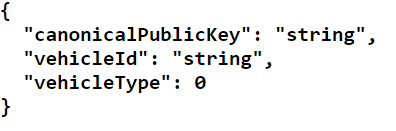
\includegraphics[width=0.5
	\textwidth]{Figures/conf_req}
	\caption{\label{fig:conf_req}Vehicle configuration request in JSON format.}
\end{figure}

\subsubsection{The end-point}
The RA service provides a POST controller dedicated to receiving the vehicle configuration requests. The first step that the RA does when it receives a configuration request is to try to save the vehicle's data in the database. However, it needs to first decode the JSON formatted data, because the request is a known DTO the RA knows how to decode it into its original objects. This is done by the \textit{DTOtoVehicle} method that exists on the RA's service layer, this method receives the request's \textit{VehicleDTO} and returns and object of \textit{Vehicle} which is a database entity containing each of the DTO's decoded attributes, and thus being more useful for the business logic. To achieve this, the \textit{DTOtoVehicle} method first decodes the base64 String canonical key to a steam of bytes and uses it to decode a \textit{PublicVerificationKey} object. The next step is to map the vehicle type to a vehicle profile name, a profile is built for a specific type of vehicle and contains generic vehicle information such as enrollment and authorization validity information. If these operations completed without generating exceptions and the requesting vehicle was not configured before, the vehicle configuration was successful and the\textit{DTOtoVehicle} method will return a new \textit{Vehicle} containing the vehicle's id, profile and canonical key, which will be stored in the RA's database under the \textit{vehicle} table as a new entry. 

\subsubsection{The response}
The next step is to respond to the vehicle with the PKI information. The response built by the RA is a \textit{ConfigResponse} DTO which always informs the vehicle of the response's origin, destination, and if the configuration was successful. Only in the positive case, the response will also contain the following PKI information: the certificate of the EA which will enrol the vehicle; the certificate of the AA that will authorize the vehicle; a list containing the certificates of all trusted AA which will allow the vehicle to trust incoming V2X messages; and the certificate of the Root CA which is the root of trust for this hierarchy. With this information the vehicle is able to request the RA for its enrollment certificate. 


\subsection{Vehicle Enrollment}
The vehicle enrollment operation can be used by configured vehicles to, as the name suggests, request a valid enrollment certificate. This operation involves the vehicle, the RA and the EA which is able to issue such certificate. During this communication, the RA has the function of assuring that the vehicle is configured and therefore authentic.

\subsubsection{The request}
Figure \ref{fig:enrol_req} illustrates the enrollment request which the API is expecting to receive. This DTO is composed of three elements: the destination representing the name of the EA which the vehicle is trying to contact, the encoded request which is an encoded \textit{EnrolmenRequest} as defined in Section \ref{requests}, finally the origin containing the vehicle's unique name (ITS identifier). For a vehicle to build the DTO which the RA is expecting to receive, it must be able to build and encode the \textit{EnrolmenRequest} element of the DTO as defined in the V2X Library. To do so, the vehicle first has to generate necessary cryptographic keys. Such keys are a new verification key pair, which the public key is to be certified by the enrollment certificate, and a symmetric AES key to encrypt the request and share with the EA. With these keys, the vehicle is able to use the V2X Library in order to generate and encode the \textit{EnrolmenRequest} data structure into a byte stream. The final step is to transform such byte stream into a base64 string and create the request DTO with the other origin and destination attributes.

\begin{figure}
	\centering
	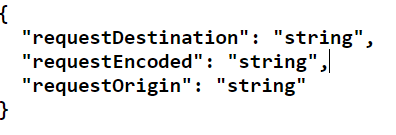
\includegraphics[width=0.5
	\textwidth]{Figures/enrol_req}
	\caption{\label{fig:enrol_req}Vehicle enrollment request in JSON format.}
\end{figure}

\subsubsection{The end-point}
The RA service provides a POST controller dedicated to receiving the vehicle enrollment requests. The first step that the RA does once it receives such request is try to verify its origin. This is done by the \text{verifySource} method which is implemented on the service layer of the RA. This method has two main functions, verifying that the vehicle is already configured within the RA, and if the destinations EA is ready to receive the vehicle's request. To do so, this method receives the request DTO as it was sent by the vehicle. First, it gets the origin of the request and queries the RA's database for that specific vehicle. In the event that the vehicle is not found, an appropriated exception will be thrown. Then using the name of the EA on the request's destination attribute, this method tries to find the such CA on the database. If found, it checks if the CA type is set to enrollment, it has signature and encryption keys, and a certificate associated. This is done to ensure that the EA that the vehicle is trying to contact is able to issue the enrollment credential. In the case that these verifications fails, an appropriate exception will be thrown. The last step is to try to decode the \textit{EnrolmenRequest} from its base64 string format into an array of bytes representing the V2X Library encoded data structure. 

Once the origin and destination of the request are verified by the RA, it is time to send the vehicle's request to the target EA. Since the PKI Manager and RA Service are part of the same project, this communication is achieved through a simple service call. The service layer of the PKI Manager provides the RA with the \textit{caService} class which contains every service which the CAs are able to provide. In this case the service needed by the RA is the \textit{validateEcRequest}, this method has the objective of validating the \textit{EnrollmentRequest} structure, therefore ultimately verifying the vehicle's identity. In order to do so, it needs to perform the following steps: decrypting the request, validating the vehicle's signatures within, and finally returning the \textit{EnrollmentResponse} which may contain the enrollment certificate. 

The RA calls the \textit{validateEcRequest} service by passing the \textit{EnrolmenRequest} and name of the EA, which were found on the vehicle's request DTO; and the vehicle's canonical key and profile name found on the RA's database under the vehicle's configuration information. In order to decrypt the request, this service first gets the stored information relative to the target EA. Using the name of the EA, it gets the EA's certificate from the PKI Manager database, and its encryption/signature key pairs from the keystore. With the EA's relevant information, this service calls the V2X Library in order to decrypt the request. This is achieved through the V2X Interface which specifies the services available by the Library side to the PKI Manager. The \textit{decryptRequest} service given the encrypted \textit{EnrolmenRequest}, the EA's decryption key (private key) and certificate will verify if the request was encrypted to that EA, and if so decrypt it using the provided private key. To do so, it first decodes the byte encoded \textit{EnrolmenRequest} into an \textit{EncryptedData} structure, then using the cryptographic module of the V2X Library calculates the hash of the EA certificate and compares it to the hash that can be found within the recipient information field of the request. If there is a match, the symmetric encryption key will be decrypted using the private key of the EA, giving access to the key which encrypted the request. To decrypt the request, this method retrieves the AES cipher text field from the request and tries to decipher it using discovered symmetric key. In case that this method fails to perform such description operations or there is no match on the calculated EA certificate hash and recipient identifier within the request, an approprieate exception will be thrown by the service. Otherwise, the signed request will be returned containing the vehicle's signatures and the requested subject attributes.

The next step that the \textit{validateEcRequest} method does is to verify the vehicle's identity. To do this, it calls the \textit{verifyEcRequest} service provided by the V2X Library to verify the vehicle's signatures. This method uses the recently decrypted request and the vehicle's canonical public key to first verify the request's outer signature, this assures the EA that the vehicle that build the request has possession of the private canonical key which was attributes to it during manufacture. The next step is to verify the request's inner signature. To do so, the Library gets the inner signed structure from the request, from this structure extracts the verification public key which the vehicle is trying to get certified by the enrollment credential, and finally verifies the inner signature. This assures the EA that the vehicle has possession of the corresponding private key, therefore making it impossible for the EA to issue an enrollment credential to a vehicle which does not have the correct verification key pair. The verification of the enrollment request is only accepted if both signatures are valid. This service returns an enrollment response code which summarizes what happened during the request's validations, some possible outputs are: OK, can't parse, not the recipient, invalid signature, incomplete request, decryption failed, etc. 

\subsubsection{The response}
The final step is to build the response to the vehicle, this is done by the \textit{genEcResponse} service of the V2X Library which is called by the PKI Manager. Since it is at this step that the enrollment credential will be generated, the PKI Manager gets from its database the profile information of the vehicle using the profile name which was sent to it by the RA. This information is necessary to issue the enrollment credential as it contains information such as the default certificate time and geographic validity. The \textit{genEcResponse} service works with the signed request; the information of the EA, including its signature key pair and certificate; the vehicle's profile information; and the enrollment response code from the last step. The first verification done by this service is with the enrollment response code, if it is a negative code such as can't decrypt, invalid signature, can't parse, etc. A new \textit{EnrollmentResponse} \ref{requests} is built without the generation of the enrollment credential. If the response is OK, this service will issue the enrollment credential. This certificate is generated using the vehicle profile information and the inner enrollment request which contains the vehicle's verification key and requested subject attributes. Once the certificate is generated by the V2X Library, the \textit{EnrollmentResponse} is generated including the enrollment credential. In both cases, response is signed by the EA's signature key and encrypted using the shared symmetric key. Such response is returned to the PKI Manager which saves the credential on its database marked as active, identified by its hash, and issued by the specific EA. The final step is to return the encrypted response to the RA which sends it to the requesting vehicle. To do so, the RA first makes the \textit{EnrollmentResponse} object ready to be transferred by encoding it in base64 text and encapsulating in a response DTO. Then the RA's controller is able to return the vehicle's expected string based object. However, if the EA was not able to retrieve the shared symmetric key from within the \textit{EnrollmentRequest}, therefore it was not able to built the encrypted \textit{EnrollmentResponse}. In this case, the RA is notified and will send the response DTO marked as failed without the EA's response structure.


\subsection{Vehicle Authorization}
The vehicle authorization operation can be used by enrolled vehicles in order to request an authorization ticket. Such operation involves the vehicle, RA, EA, and the AA. As in the previous operations, the responsibility of the RA is to assure that the requesting vehicle is configured, and also decoding the string based request DTO so that they can be used by the PKI Manager's services.

\subsubsection{The request}
Figure \ref{fig:auth_req} illustrates the authorization request which the API is expecting to receive. This DTO is similar to the one expected by the enrollment end-point, the only differences are the encoded request which is an \textit{AuthorizationRequest} as defined in Section \ref{requests}, and the destination references the AA which will authorize the vehicle. To generate and encode such a request, the vehicle is able to use the V2X Library, it just needs to generate the necessary keys first. Such keys are a new verification key pair which will be certified by the authorization ticket, and two different symmetric keys in order to share with the EA and AA. Like the previous operations, the string based DTO forces the vehicle to be able to encode such \textit{AuthorizationRequest} in order to create the request which the RA is expecting.

\begin{figure}
	\centering
	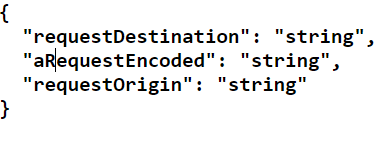
\includegraphics[width=0.5
	\textwidth]{Figures/auth_req}
	\caption{\label{fig:auth_req}Vehicle enrollment request in JSON format.}
\end{figure}

\subsubsection{The end-point}
The RA service provides a POST controller dedicated to receiving the vehicle authorization requests. The first step that the RA does once it receives such request is to try to verify its origin, this is done by the same \text{verifySource} method used in the enrollment operation. However, in the authorization operation the RA processes this step differently. As explained in the authorization protocol \ref{protocol}, the authorization process of a vehicle is composed of multiple individual authorization requests, each for an authorization ticket. Through this first step, the RA has the responsibility of determining if the received request is the first of the vehicles' authorization process or not. The \text{verifySource} method receives the request DTO as it was sent by the vehicle, after validating that the destination AA is ready to issue certificates it validates that the origin vehicle is configured in the RA. If the vehicle is found, then this method gets the maximum number of authorization requests that the vehicle is allowed to make from its profile information. Comparing this number to the number of requests done by this vehicle (identified by the origin on the request DTO) allows the RA to know if the received request is the first of the authorization process, and therefore if the vehicle's enrollment needs to be validated, see Figure \ref{fig:protocol_2}. To protect against vehicles using other vehicle's identifiers to request authorization tickets the SSL protocol is used. The communication security provided by the protocol allows to the RA to trust that the vehicles are in fact the ones that their secret identifier say they are. When a vehicle starts the authorization process it is expected by the RA that all the underlying requests will be done close to each other, in a sequence manner. However, if this is not the case it would be necessary to implement a cron based mechanism that after some time marks the vehicle so that the RA knows that its enrollment must be verified in the next authorization request regardless of the request counter. The last step done by this method is to try to decode the \textit{AuthorizationRequest} from its base64 string format into an V2X Library data structure. 


Once the RA has verified the origin, destination and determined the enrollment validation for the request, it is time to send the decoded request to the AA. To do so, the RA calls the \textit{validateAtRequest} on the CA's service layer. From all the services which the CA's are able to provide to the RA, this method can be seen as the service which the AA provides for the RA to send the vehicle authorization requests. Such method has the objective of validation the \textit{AuthorizationRequest} structure. To do so the following steps are performed: decrypting the request, validating the vehicle's signature, requesting the verification of the vehicle's enrollment if applicable, and finally generating the \textit{AuthorizationResponse} which may contained the issued authorization ticket.

The RA calls the \textit{validateAtRequest} by passing the \textit{AuthorizationRequest}, the name of the AA, the vehicle's profile name, and the flag that determines if the vehicle's enrollment is to be verified or not. The decryption of the request is similar to the process used by the vehicle enrollment operation: the \textit{validateAtRequest} service starts by getting the AA's certificate and keys from the database and keystore. With this information it calls the same V2X Library \textit{decryptRequest} service which returns the signed request structure. With the decrypted request the AA is able to verify the vehicle's signature using the to be certified public verification key in the request. Such validation assures the AA that the vehicle which created the request has possession of the corresponding private key. In the eventuality that request is not valid because, for example, the request is badly formed, it was not encrypted to this AA, the signature is invalid, etc the response code to be delivered to the vehicle in the response will be of error.

\subsubsection{The response}
If the response code is positive and the enrollment validation flag was set to true by the RA in the last step, the next step is to request the EA for the validation of the vehicle's enrollment. This is done by first extracting the \textit{AuthorizationValidationRequest} structure from the now decrypted \textit{AuthorizationRequest}, the \textit{AuthorizationValidationRequest} structure contains the EA encrypted vehicle's enrollment signature and the shared request. The AA is able to find the hash of the EA's certificate within the shared request. With this information it is able to get the name of the EA from the database and send it the \textit{AuthorizationValidationRequest} by calling the \textit{validateEnrollment} CA service. In the case that the RA determined that the request is not to be enrollment verified, the call to the EA's \textit{validateEnrollment} service is skipped, 


The first step that this EA service performs is the decryption of the received request, to do so, it relies on the name of the EA to get its certificate and decryption key from the persistent layer of the PKI Manager. Once the decryption parameters are set, it calls the V2X library \textit{decryptRequest} service to decrypt the request. The next step is for the EA to validate the vehicle's enrollment by verifying its enrollment certificate and signature. First, this service gets the vehicle's credential from the database (stored by the EA at the enrollment phase) and checks if it is still marked as valid, if this is the case, then the service cryptographically validates the enrollment credential using the \textit{verifyCertificate} service provided by the V2X Library. This service, given a certificate and the corresponding certification chain will verify if such certificate belongs in that chain by decrypting its signature using the public verification key of the next certificate in the chain, in addition to this, it also validates the expiration date on the certificate. The return value is a simple boolean which, if true, allows the EA to continue with the vehicle's enrollment validation by decrypting its enrollment signature. This process can be started by calling the V2X Library \textit{verifyEnrollmentSignature} service which given the vehicle's enrollment credential and \textit{AuthorizationValidationRequest} is able to extract the enrollment signature from the request and verify it using the credential's public key. If the signature is valid the EA has validated the vehicle's enrollment and returns a positive response to the AA. In the case either the credential or the signature is not valid, a negative response will be sent yo the AA. 

The final step is to build the response to the vehicle which may contain the requested authorization ticket. To generate such response the AA, first gets its signature key pair; its certificate; the vehicle's profile information; the signed request; and the response code which resulted from the validation of such request and, if applicable, the vehicle's enrollment. With this information, the AA calls the \textit{genAtResponse} V2X service which is the response code is positive will issue the authorization ticket using the AA's certificate, private signature key and vehicle's profile information, including it in the response. The response structure is generated always signed by the AA and encrypted to the vehicle, (using the same symmetric key from the request). The final step is to return this response to the RA marked as positive so that it can be returned to the vehicle.


\section{Vehicle Manager}
The Vehicle Manager has the responsibility of generating client vehicles for the PKI Manager, at a high level we can see the Vehicle Manager as a vehicle manufacturer which is trusted by the RA service. In addition to generating the vehicles, it is this component's responsabilty to provide a V2X environment where the generated vehicles are able to communicate with each other. To ease the testability of such environment, the Vehicle Manager reads the application properties to load the execution variables, such as the number of vehicles, number of times a AT is used, pattern of certificate usage, etc.

At this point we have a REST API which is documented using the Swagger tool, Although the automatic and interactive documentation is useful in its own way, the main reason why we chose Swagger to document our the RA Service is the possibility of automatically generating client libraries for the API. For this purpose, we used the \textit{Swagger Codegen} tool, an open source project available on the \textit{GitHub} repository. This tool works with the URL of our API's documentation and is able to generate a client project where the communication layer is made to specifically communicate with the API. This allowed us to save time abstracting from the communication details and focus on the functionality of the Vehicle Manager.

The Vehicle Manager is a simple multi-threaded \textit{Java} project which can be started using the \textit{Main} method. The first operation done by this method is to initialize the generation of vehicles, which is managed by other class. The output of the vehicle generator is a list containing the vehicles, each with a fixed size random \textit{String} as the identifier, and one of the V2X library supported encryption/signature algorithms. At this point the main method knows how many vehicles will participate in the execution so it populates each vehicle with a list of its neighbours. 

The multi-thread attribute of the Vehicle Manager comes into play right after the generation of the vehicles, where each vehicle represents a different thread in the execution of the application. Our objective with this is to make the V2X communications seem more realistic where each vehicle is sending messages to its peers in no particular order, resutling in different communication situations. 

The execution of the threads starts when the main method calls the \textit{start} method of the generated vehicles. When started, each vehicle performs the protocol described in Section \ref{protocol} by requesting the operations of the RA Service of vehicle configuration, enrollment and authorization. Using the V2X Library enables each vehicle to generate the most complext request elements. The result of the protocol is the installation of the CA certificates, the enrollment credential and a list of authorization tickets within each vehicle. 

Once a vehicle has all the needed certificates it is time to start communicating with its peers. To do so, it starts two timers: the \textit{CAMtimer} and the \text{includeCertTimer}. The first has the responsability of periodically sending CAMs, each time electing an authorization ticket to sign the message (currently used AT). The second timer informs the vehicle when it is time to send the full authorization ticket within the signer information of its next message so that it can be distributed. 

The process of broadcasting a CAM is composed of three steps: checking for unknown authorization tickets, generating the message, and sending it. In the first step the vehicle searches its internal list of unknown authorization tickets, if any hash is found then it will be included in the next CAM so that the corresponding full certificate can be requested. The generation of the CAM itself is done using the V2X Library with respect to the currently used AT, the corresponding signature keys, the list of unknown ATs, and wether to include the full signing AT or its hashed reference. Finally, in order to send the CAM the vehicle simply iterate through the list of neighbour vehicles calling their respective \textit{receiveCAM} method.
 
When a vehicle receives a CAM the first step is to look for the hash of its currently used AT within the list of requested certificates. If found, then the vehicle sets a variable to include its full AT on the next message. This mechanism allows the distribution of the currently used AT in the cases that other vehicles have requested it.
The next step is to try to verify the message. For this purpose, the vehicle first reads the message signer identifier in onder to understand the type of signature, i.e. if the message includes the signer's AT or the hash value. 

In the first case, the vehicle verifies the signer's AT against the certificates of the trusted authorization authorities. If the AT is signed by a trusted authorization authority, the vehicle stores it as trusted in a hash map enabling access on future communications, and proceeds to verify the message. This is a simple process where the signature is verified against the signer's AT, and the message generation time is within the certificate's expiration period.

In the case that the vehicle receives a CAM containing the hashed AT, the vehicle starts the verification of the message by looking for that digest on its trusted AT hashmap. If the hash is found it means that the AT was already verified and roots to a trusted AA certificate, so the message is able to be verified using the same method as in the previous case. However, if the AT is unknown the vehicle adds the digest to the list of unknown ATs so it can be requested in the next message. Because the message was not able to be verified due to the missing AT, it is stored in a list of pending messages which await verification until the full signing AT is included within an incoming CAM.

When a vehicle receives a CAM containing the full certificate it can be the consequence of this vehicle's request for an unknown certificate. Therefore, the vehicle tries to verify both the new and pending messages. For each pending CAM we compare the digest on the signer identifier to the digest of the received AT. A match means that the pending message was signed by that same AT, which is trusted by the vehicle, enabling the verification of the message.

\section{Summary}
In this chapter we presented our solution to the problem of implementing a PKI solution that allows a V2X environment while preserving the privacy of the vehicles. We started by overviewing the architecture of the solution, learning about its main components: PKI Manager, V2X Library and Vehicle Manager. We studied how such components are organized in a client-server architecture, assuming the PKI Manager as the server and the Vehicle Manager as the client. In addition, we saw that these two components communicate through the API of the server, the RA Service and utilize the V2X Library in order to generate the necessary messages. We concluded this chapter by presenting the detailed implementation of each component, where we also explained the technologies and external libraries adopted in order to implement our components. In the next chapter we perform an experimental evaluation to our V2X system, where we test the performance of the server, the resource usage of the client and finalize by discussing the security and privacy properties achieved. 

 
%%%%%%%%%%%%%%%%%%%%%%%%%%%%%%%%%%%%%%%%%%%%%%%%%%%%%%%%%%%%%%%%%%%%%%%%
